\chapter{LAMPIRAN}
\label{chap:lampiran}

\section*{Hasil Simulasi Saat Ini}
\label{sec:hasil-simul-existing}

\begin{figure}[!ht]
    \centering
    % First row - two images side by side
    \begin{subfigure}{0.48\textwidth}
        \centering
        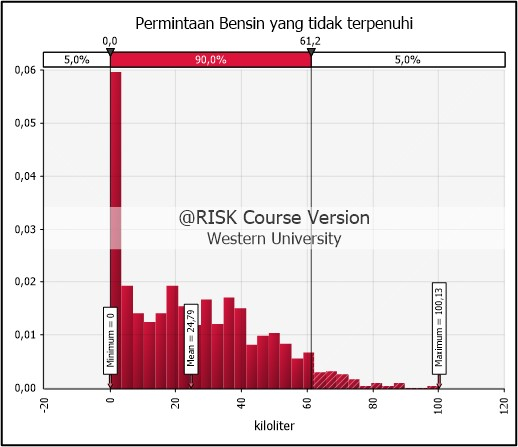
\includegraphics[width=\textwidth]{grafik/minus-bensin-saat-ini.jpg}
        \caption{Bensin}
        \label{fig:minus-bensin-saat-ini}
    \end{subfigure}
    \hfill
    \begin{subfigure}{0.48\textwidth}
        \centering
        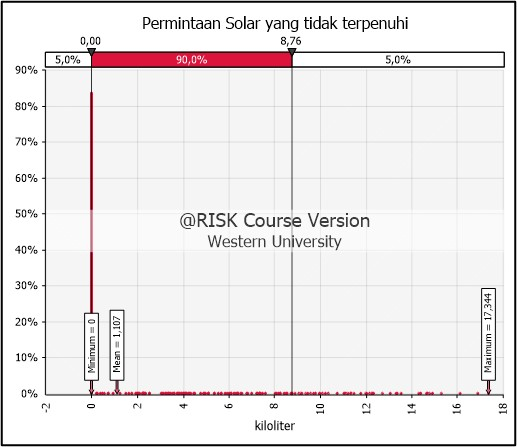
\includegraphics[width=\textwidth]{grafik/minus-solar-saat-ini.jpg}
        \caption{Solar}
        \label{fig:minus-solar-saat-ini}
    \end{subfigure}
    
    \vspace{1cm}  % Add vertical space between rows
    
    % Second row - single image centered
    \begin{subfigure}{0.5\textwidth}
        \centering
        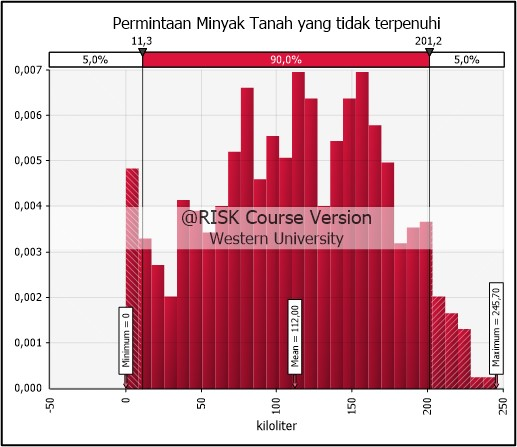
\includegraphics[width=\textwidth]{grafik/minus-mt-saat-ini.jpg}
        \caption{Minyak Tanah}
        \label{fig:minus-mt-saat-ini}
    \end{subfigure}
    \caption*{Permintaan BBM yang Tidak Terpenuhi Saat Ini}
    \label{fig:minus-bbm-saat-ini}
\end{figure}

\begin{figure}[!ht]
    \centering
    \begin{subfigure}{0.48\textwidth}
        \centering
        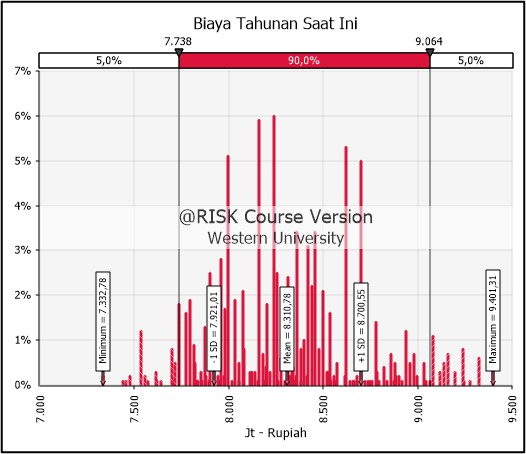
\includegraphics[width=\textwidth]{grafik/biaya-tahunan-saat-ini.jpg}
    \end{subfigure}
    \hfill  % This adds horizontal spacing between images
    \begin{subfigure}{0.48\textwidth}
        \centering
        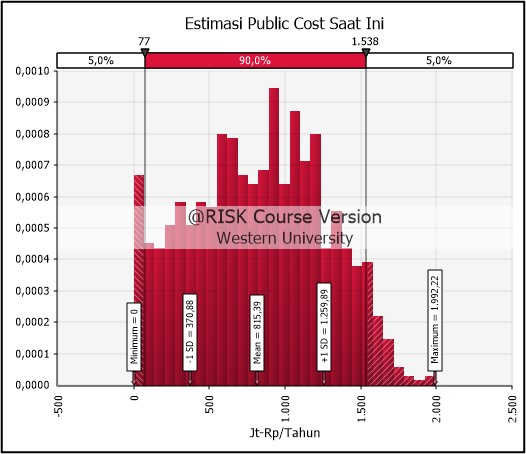
\includegraphics[width=\textwidth]{grafik/biaya-publik-saat-ini.jpg}
    \end{subfigure}
    \caption*{Hasil Simulasi Biaya Saat Ini}
    \label{fig:biaya-saat-ini}
\end{figure}

\section*{Kurva Stabilitas SPOB}
\label{sec:kurva-gz-spob}

\begin{figure}
    \centering
    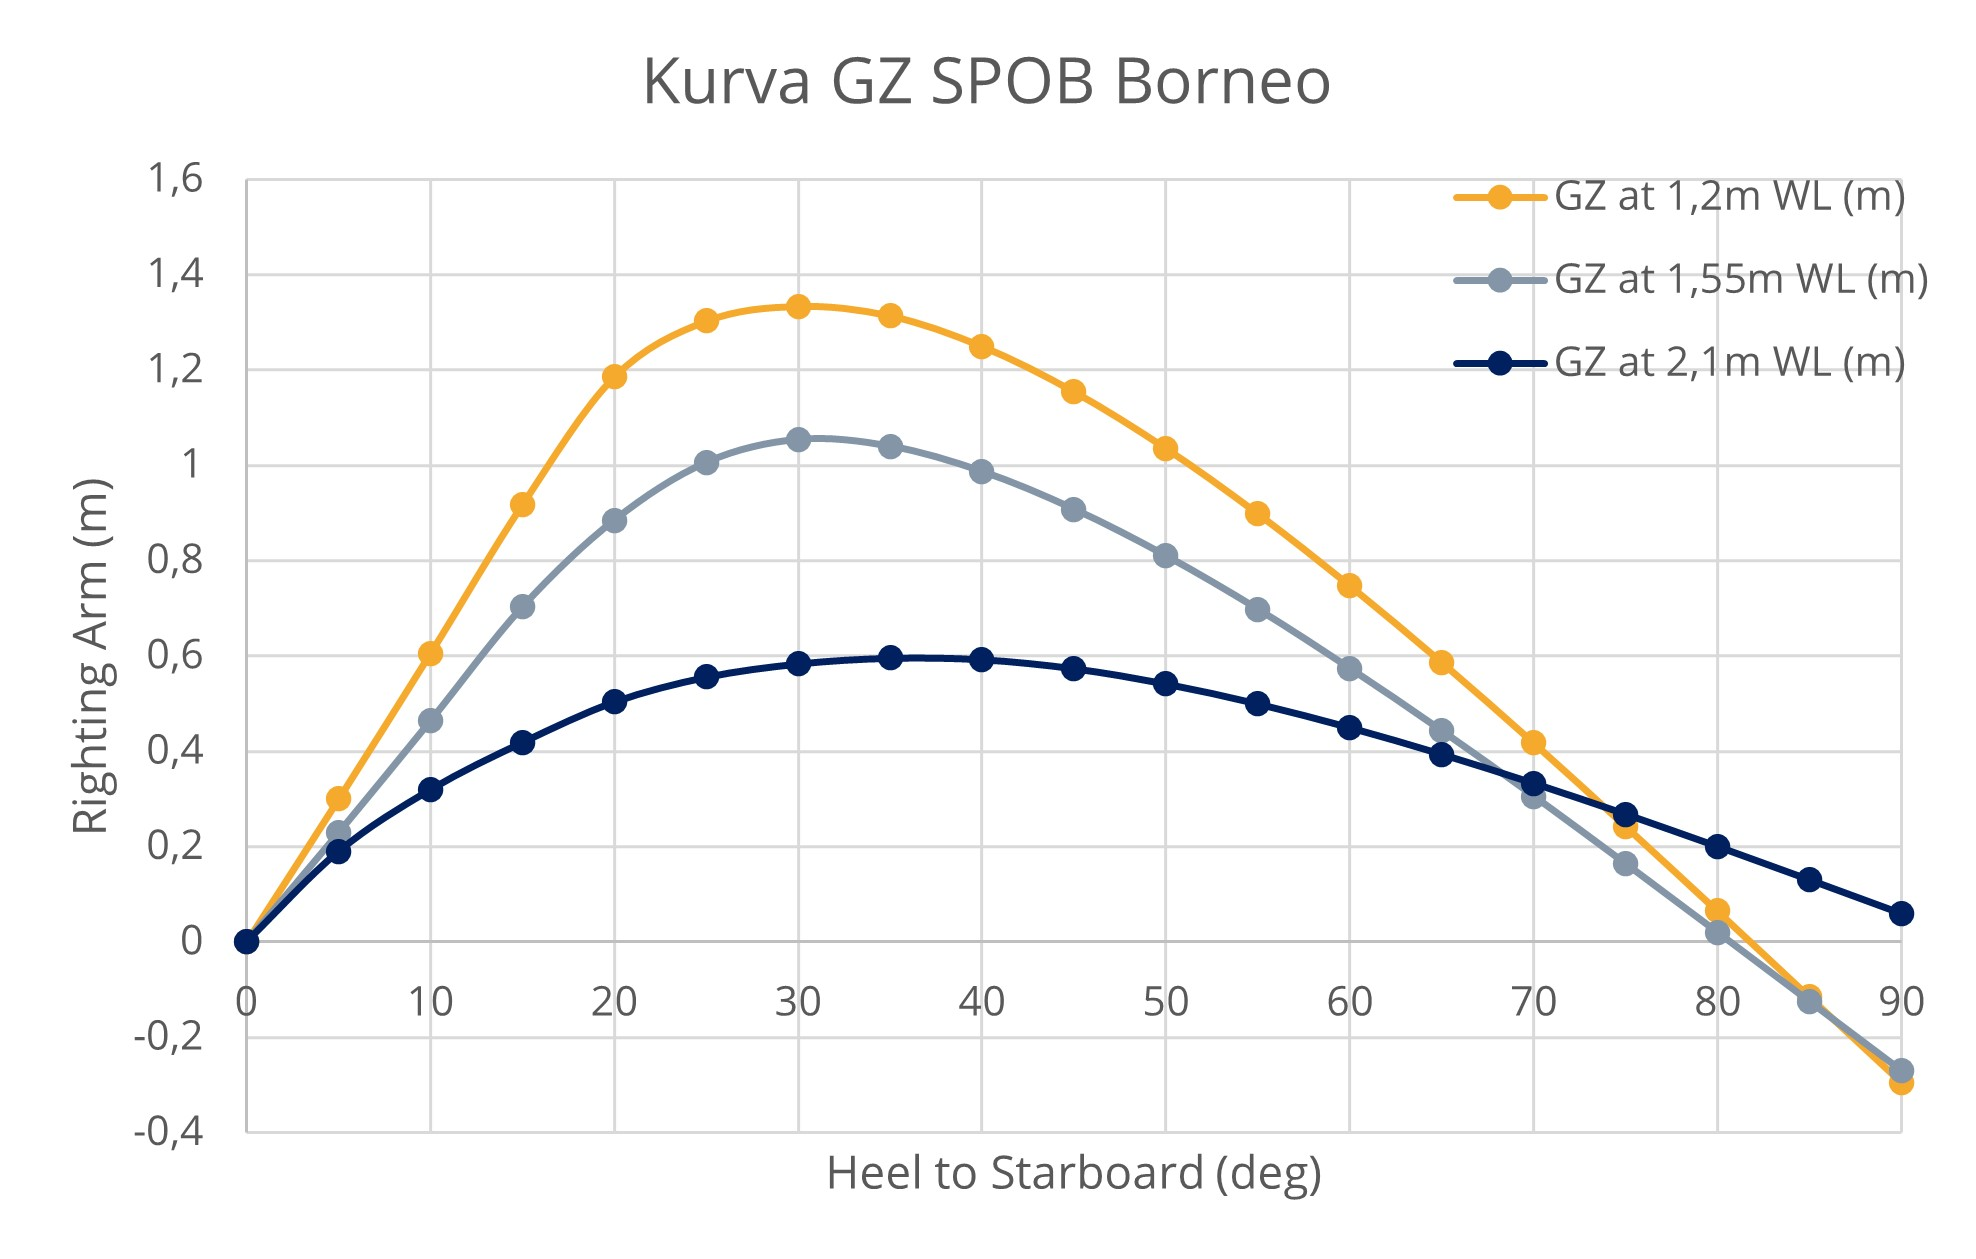
\includegraphics[width=0.7\textwidth]{grafik/kurva-gz-spob.jpg}
    \caption*{Kurva GZ SPOB Borneo}
    \label{fig:kurva-gz-spob}
\end{figure}

\newpage

\section*{Rencana Garis}
\label{sec:rencana-garis}

Gambar akan dilampirkan dalam kertas A3


\section*{Rencana Umum}
\label{sec:rencana-umum}

Gambar akan dilampirkan dalam kertas A3

\section*{Contoh Hasil Simulasi}
\label{sec:contoh-hasil-simulasi}

\begin{figure}
    \centering
    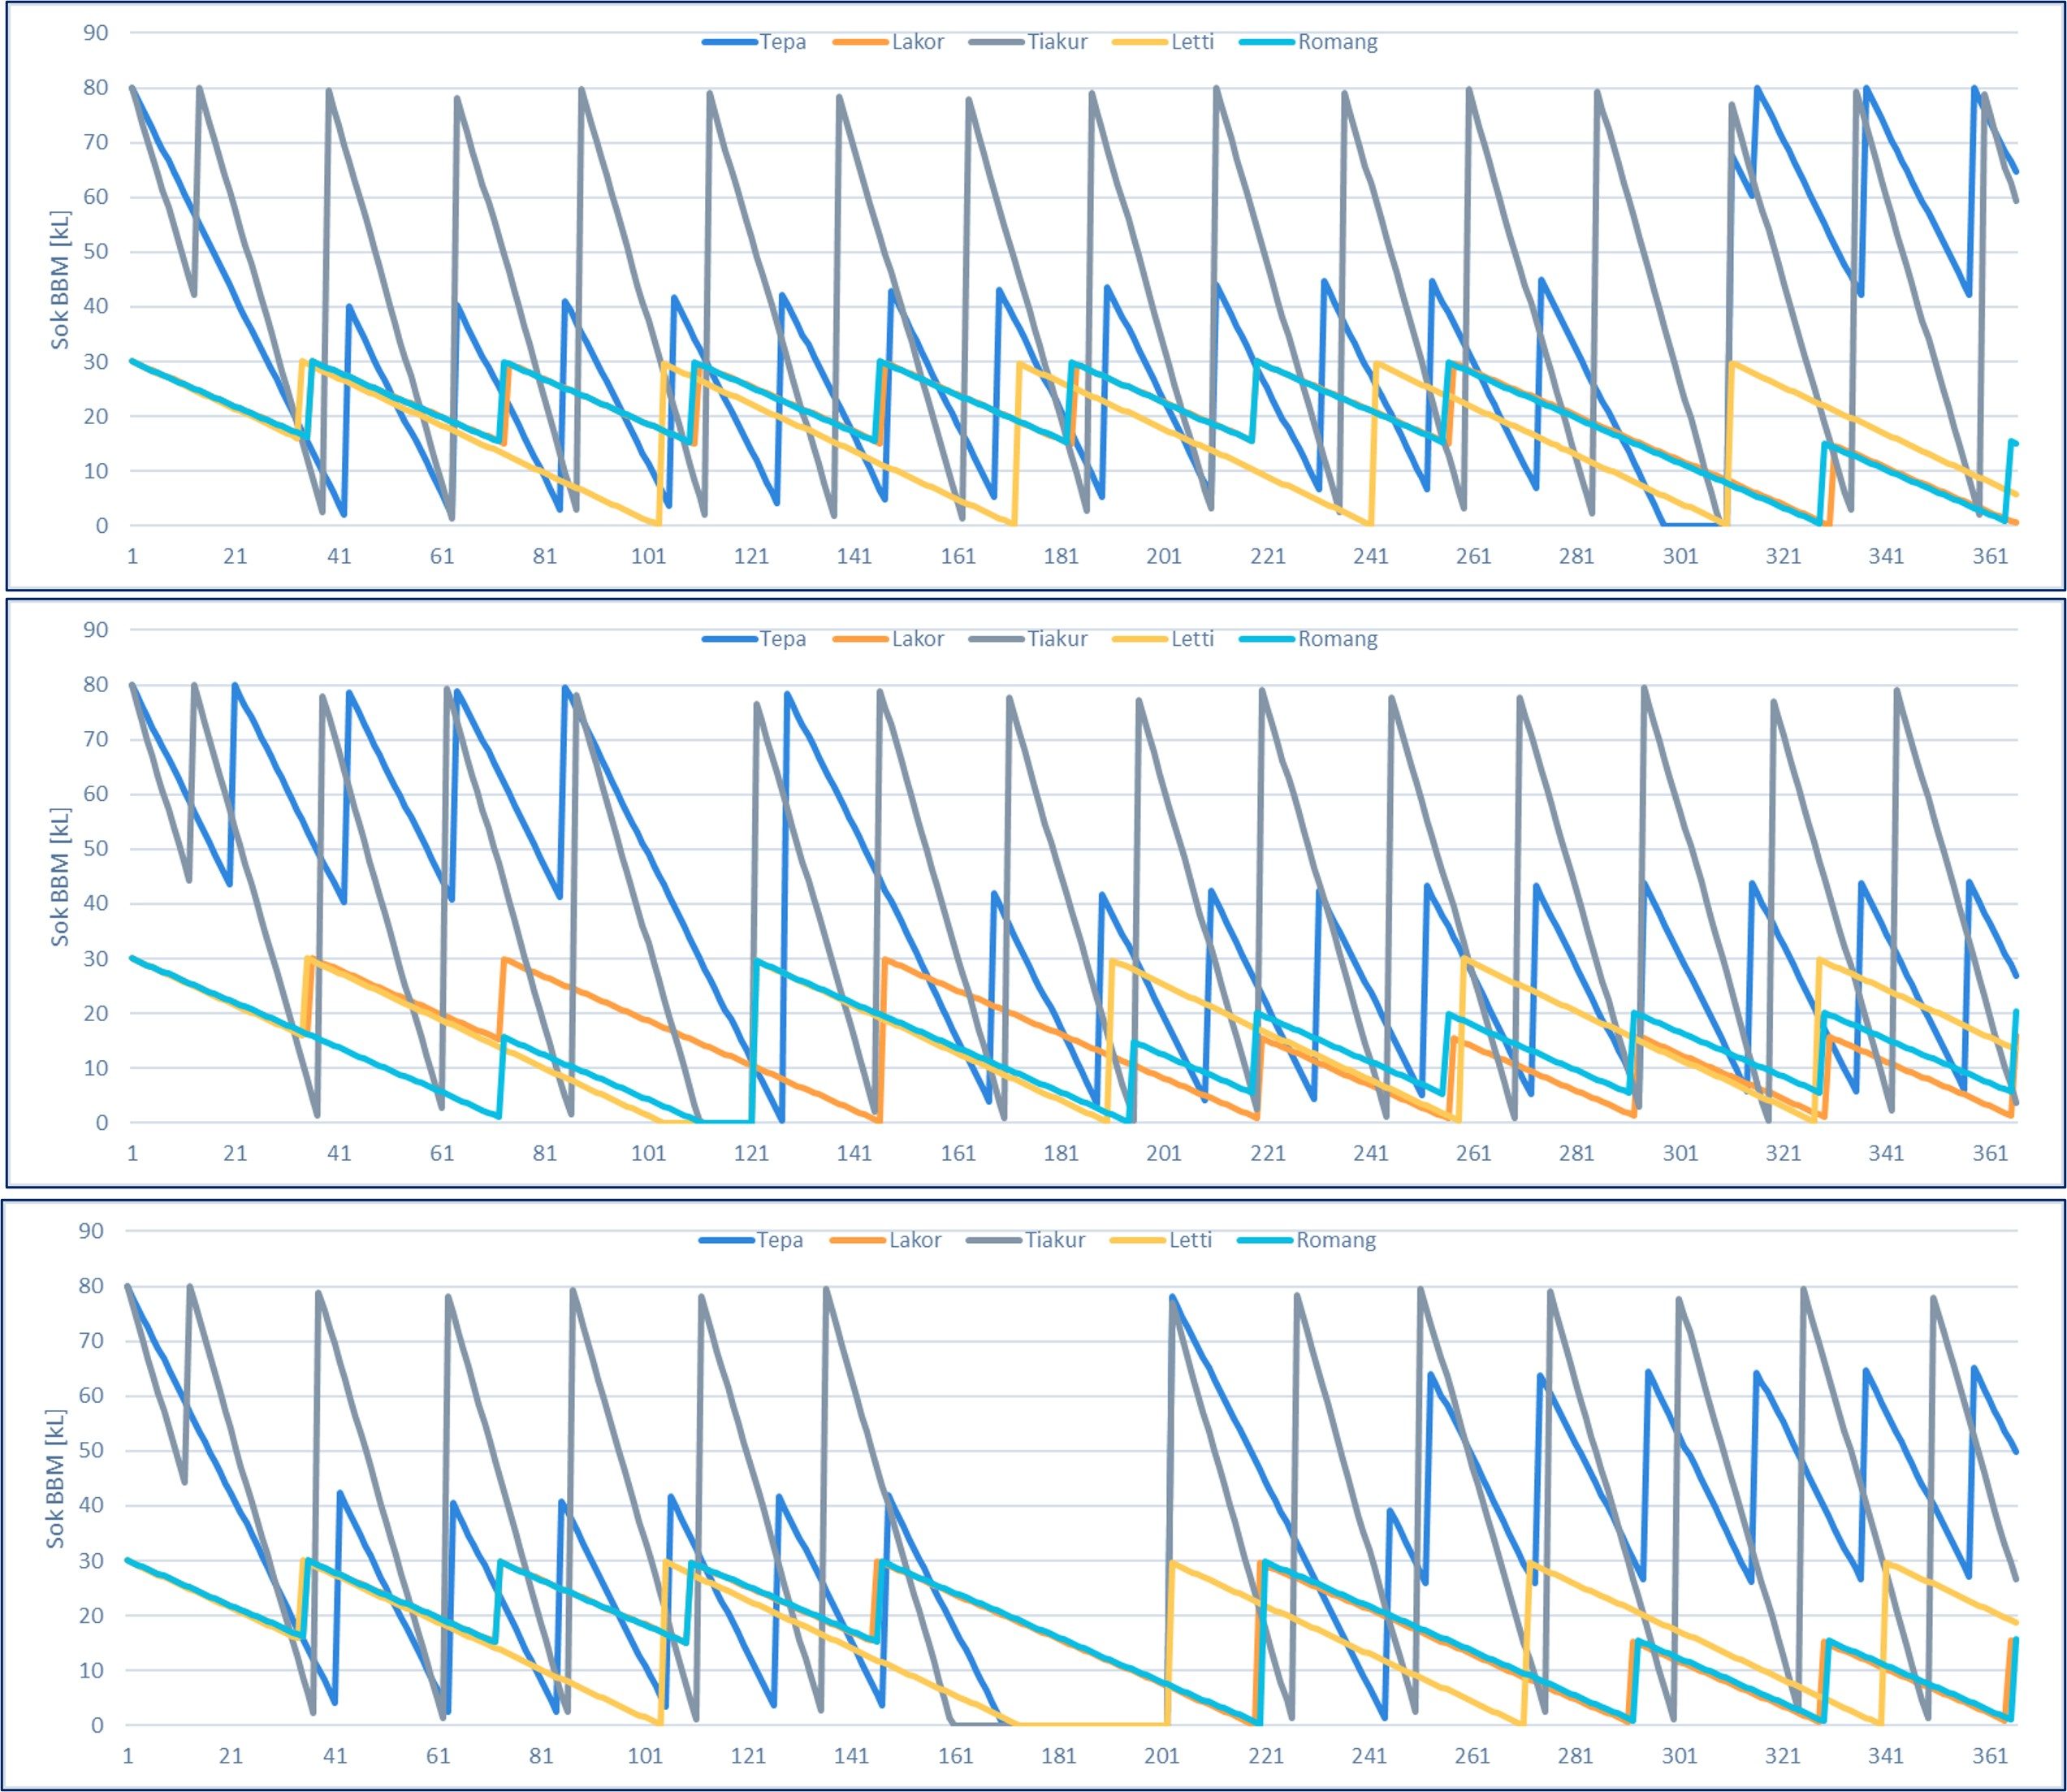
\includegraphics[width=0.9\textwidth]{grafik/contoh-hasil-simulasi.jpg}
    \caption*{Contoh Hasil Simulasi}
    \label{fig:contoh-simulasi}
\end{figure}

\newpage


\section*{Contoh Skenario Pemuatan}
\label{sec:contoh-skenario-pemuatan}

berikut adalah beberapa contoh pemuatan yang digunakan oleh kapal baru.

\begin{figure}
    \centering
    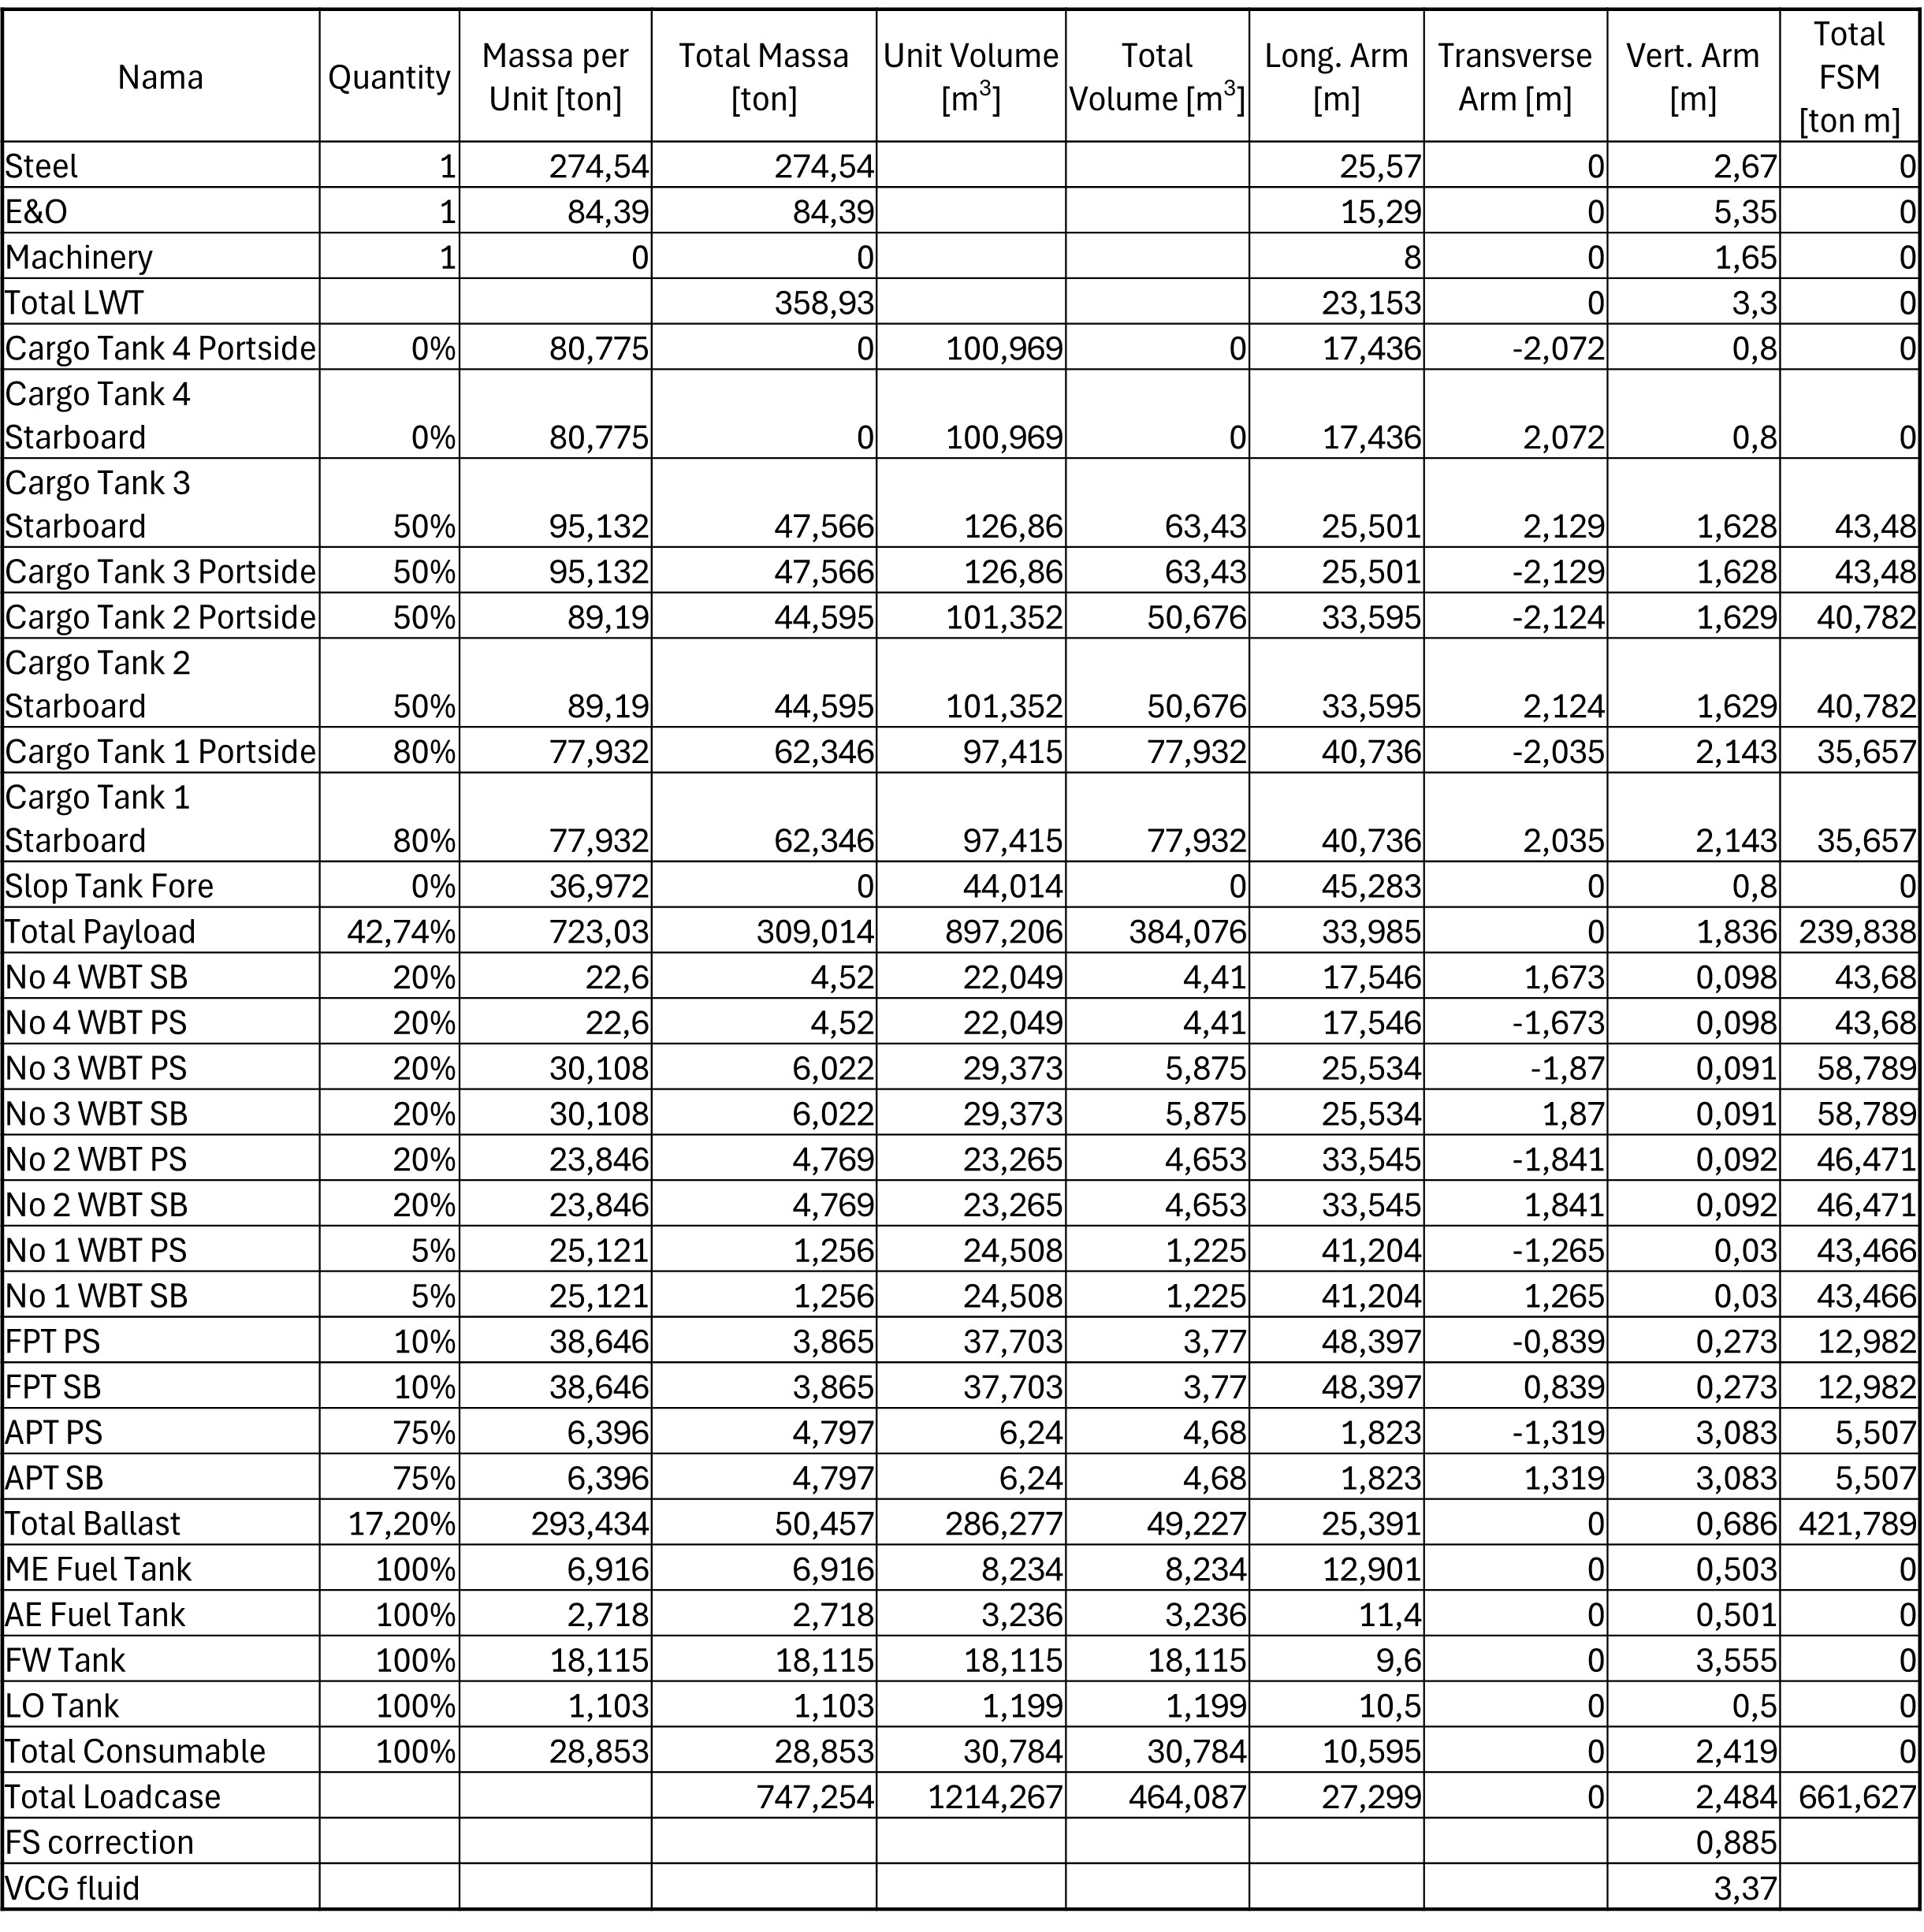
\includegraphics[width=0.8\textwidth]{grafik/tabel-pemuatan-1.jpg}
    \caption*{Tabel Skenario Pemuatan 1}
    \label{fig:contoh-skenario-pemuatan-1}
\end{figure}

\begin{figure}
    \centering
    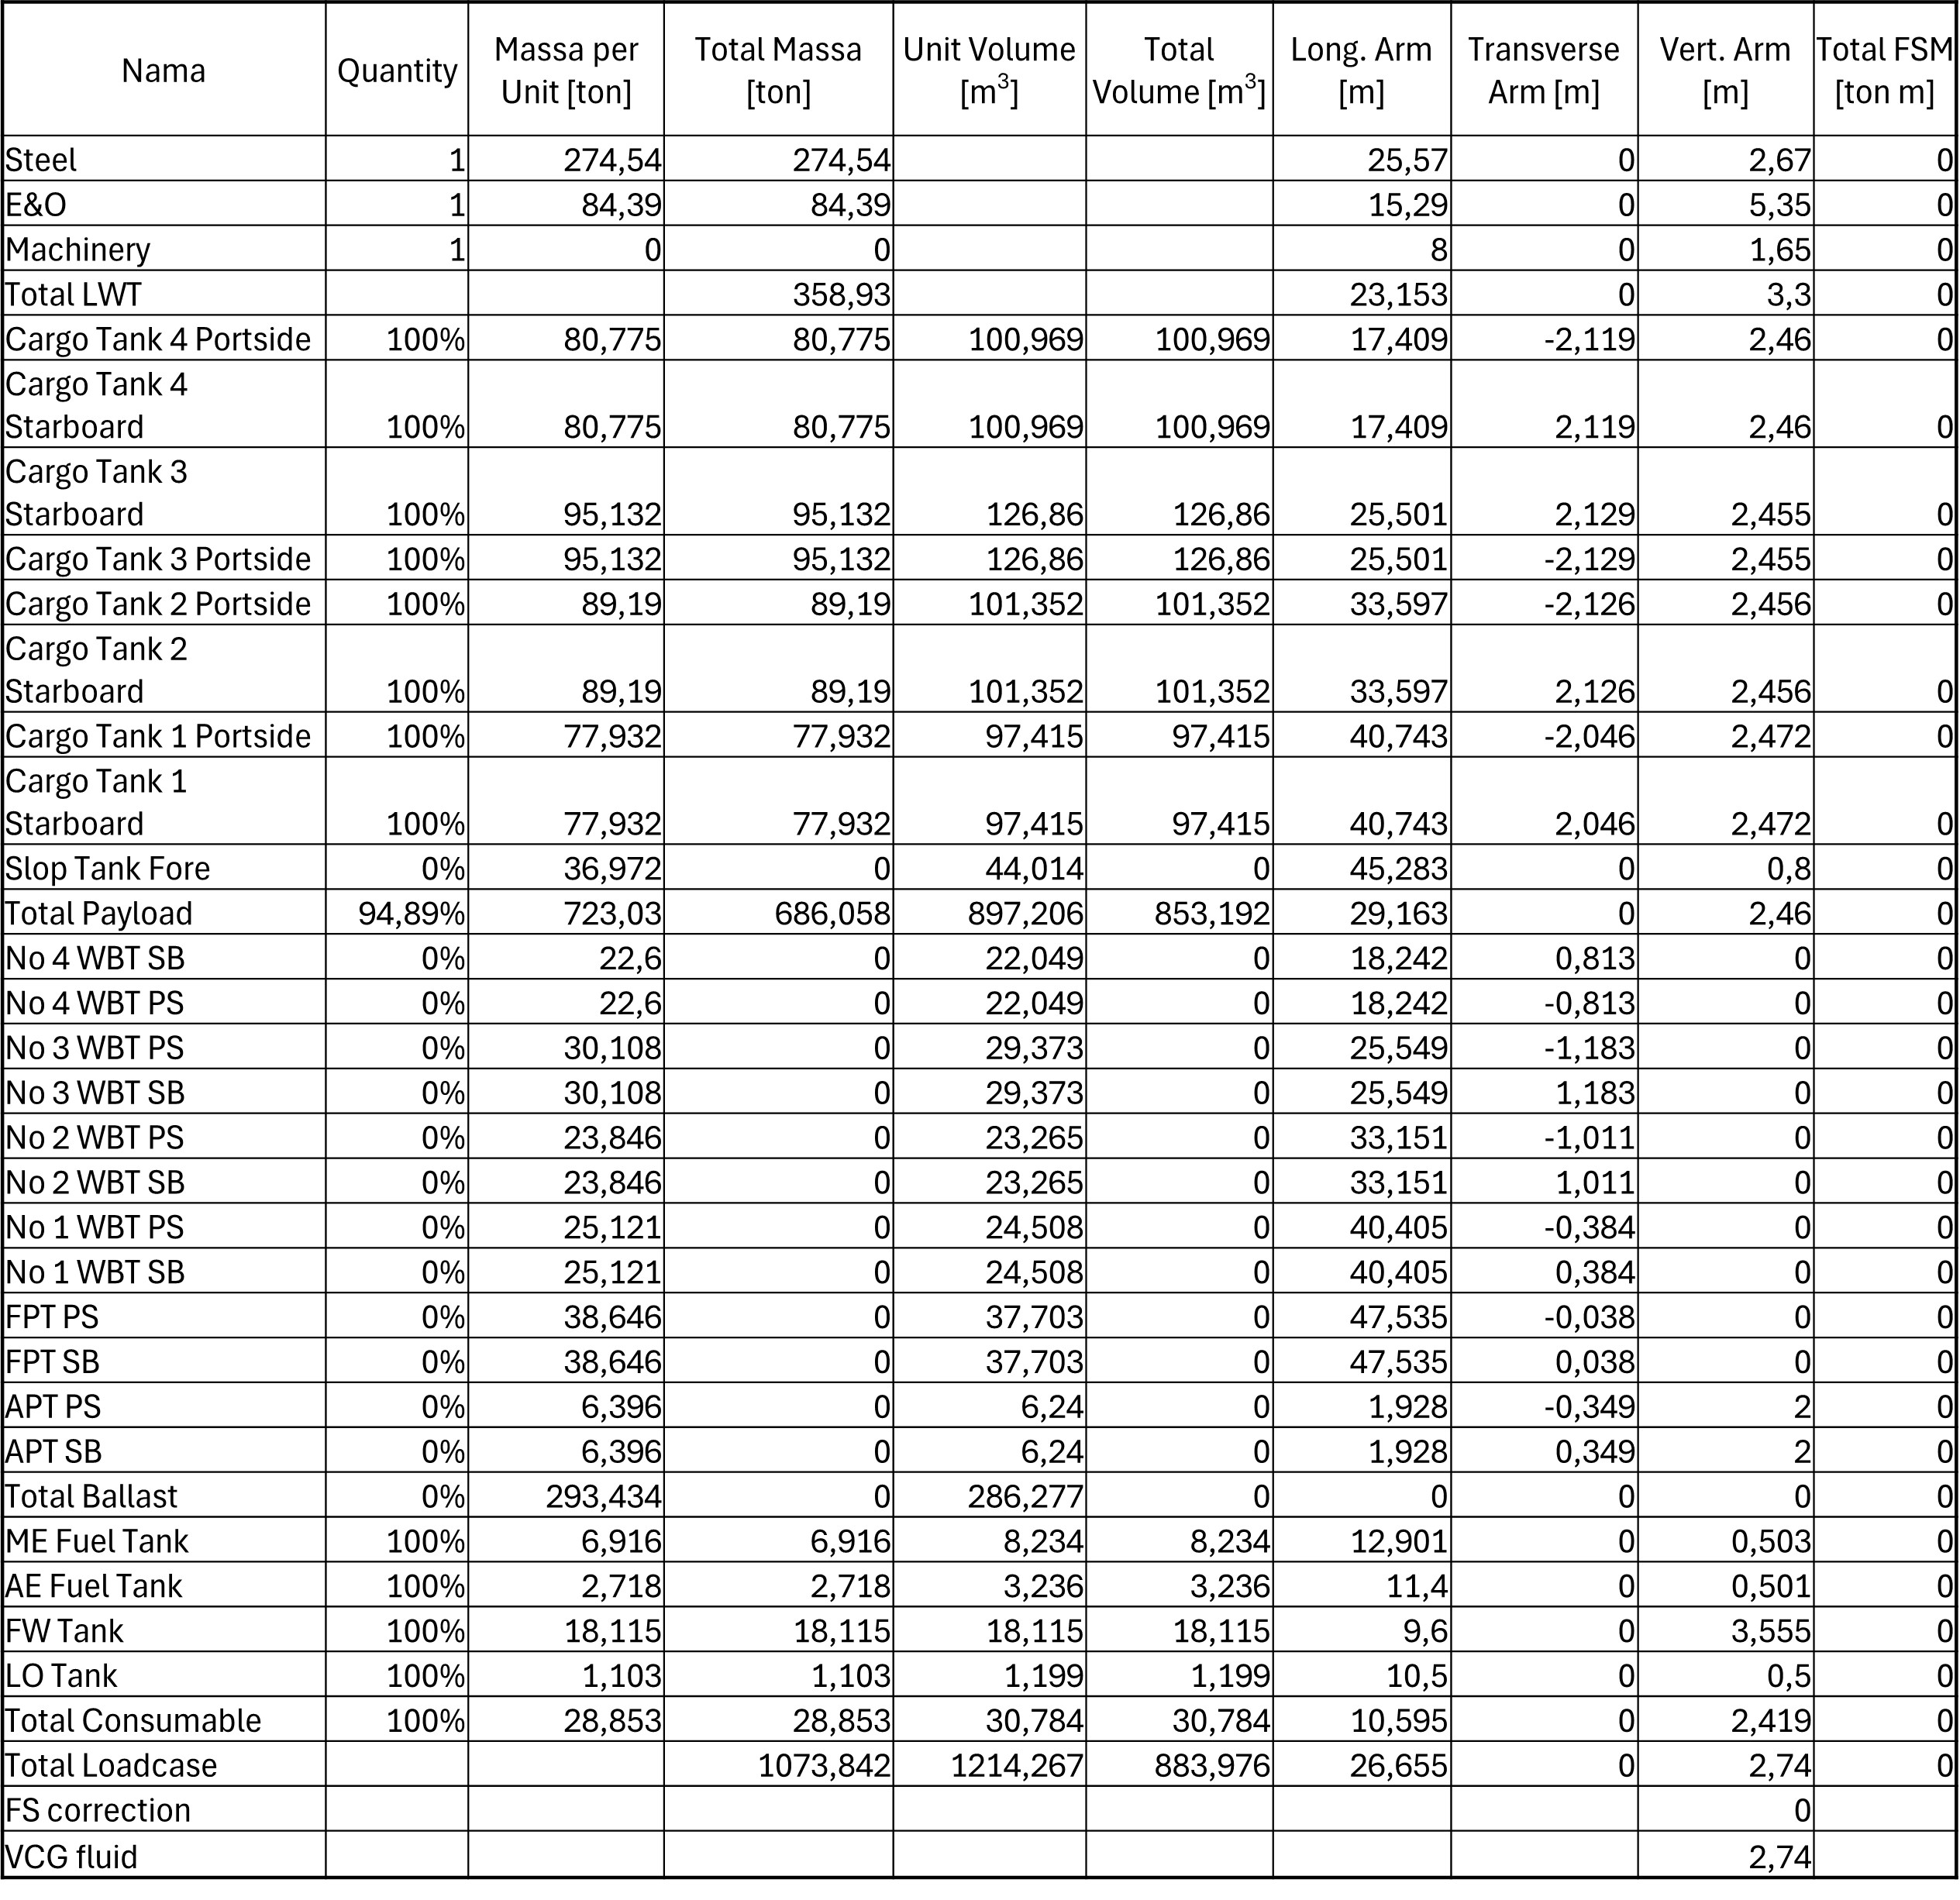
\includegraphics[width=0.8\textwidth]{grafik/tabel-pemuatan-2.jpg}
    \caption*{Tabel Skenario Pemuatan 2}
    \label{fig:contoh-skenario-pemuatan-2}
\end{figure}

\section*{Perhitungan Perancangan Kapal}
\label{sec:itungan-deskap}

\begin{figure}{!ht}
    \centering
    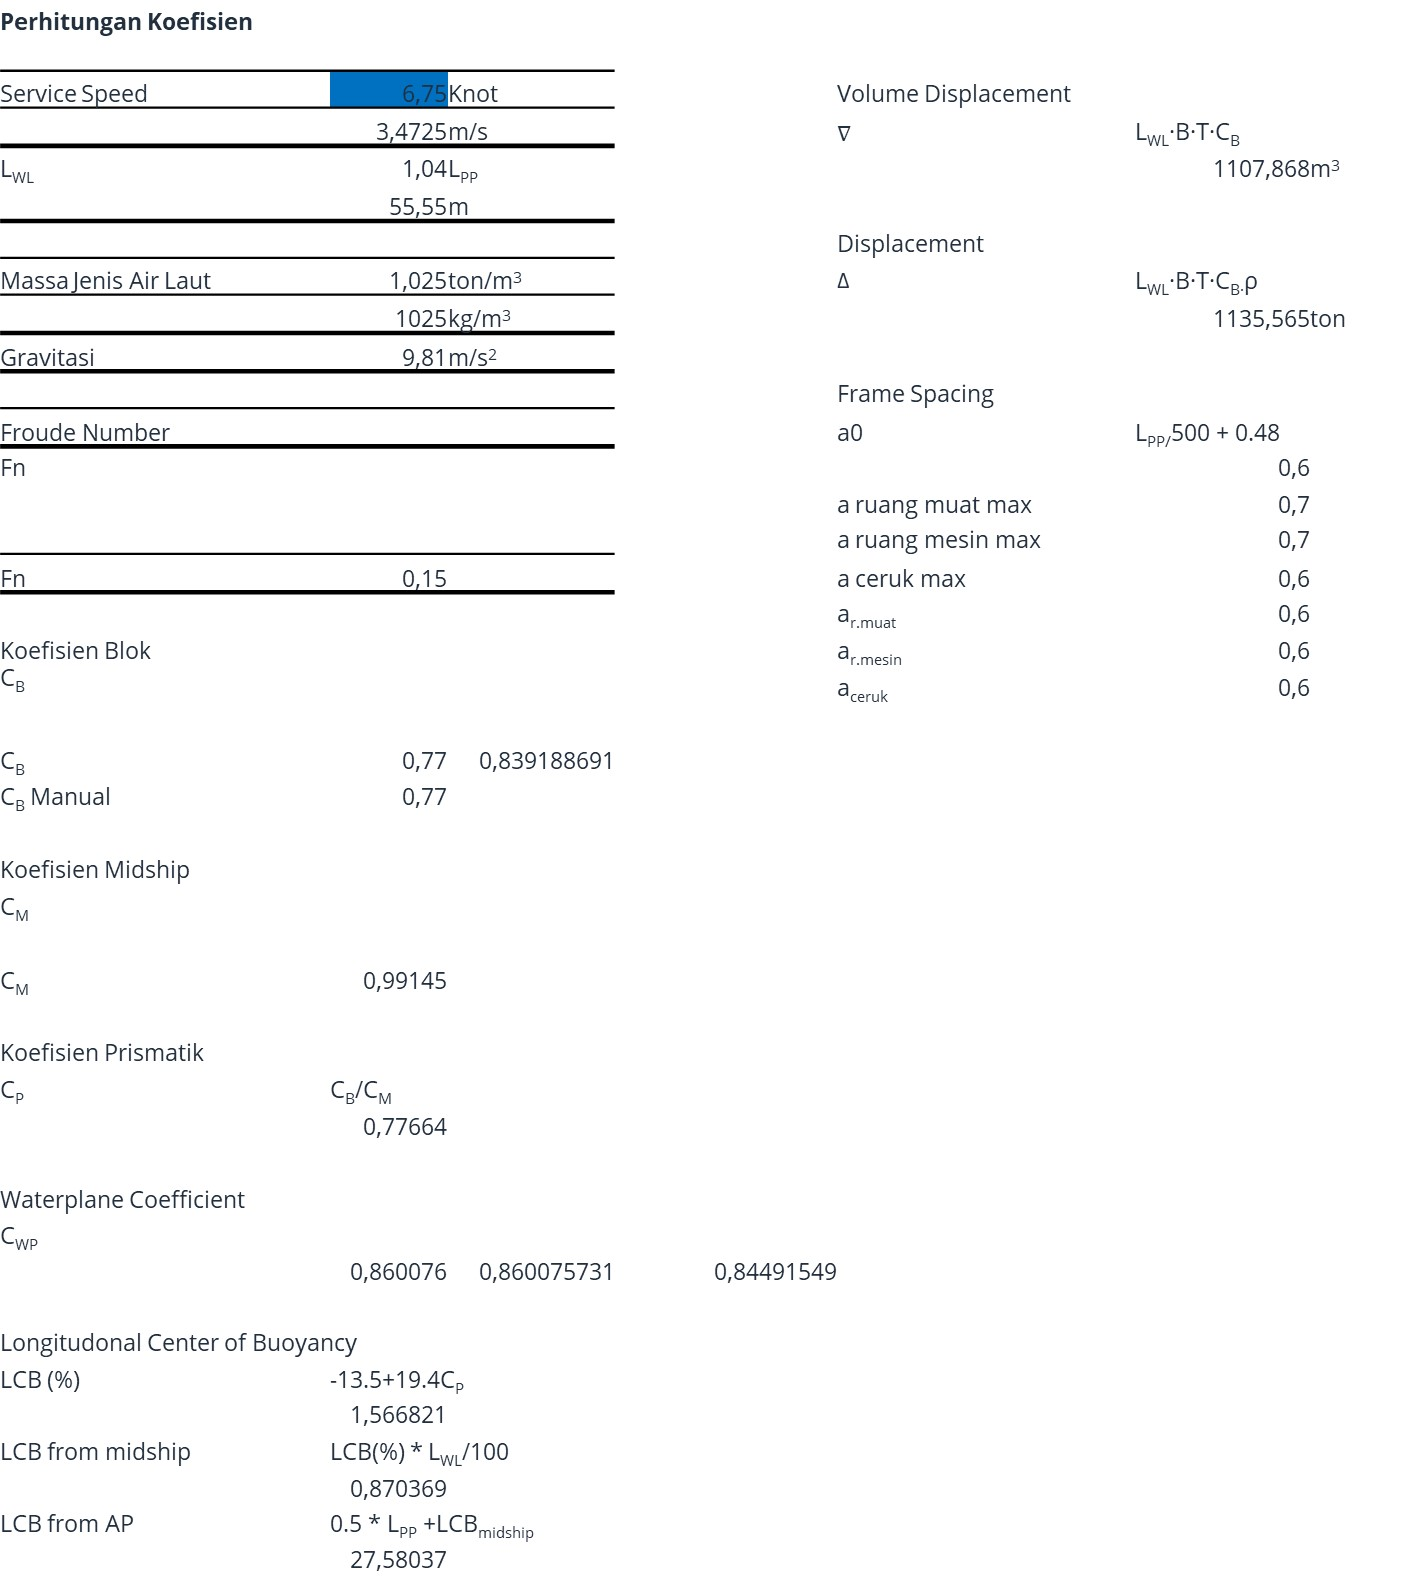
\includegraphics[width=0.8\textwidth]{lampiran/deskap-1.jpg}
    \caption*{Perhitungan Koefisien}
\end{figure}

\begin{figure}[!ht]
    \centering
    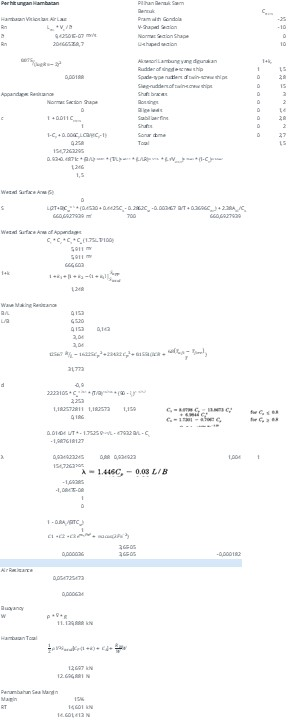
\includegraphics[width=\linewidth,height=\textheight,keepaspectratio]{lampiran/deskap-2.jpg}
    \caption*{Perhitungan Hambatan}
\end{figure}

\begin{figure}[!ht]
    \centering
    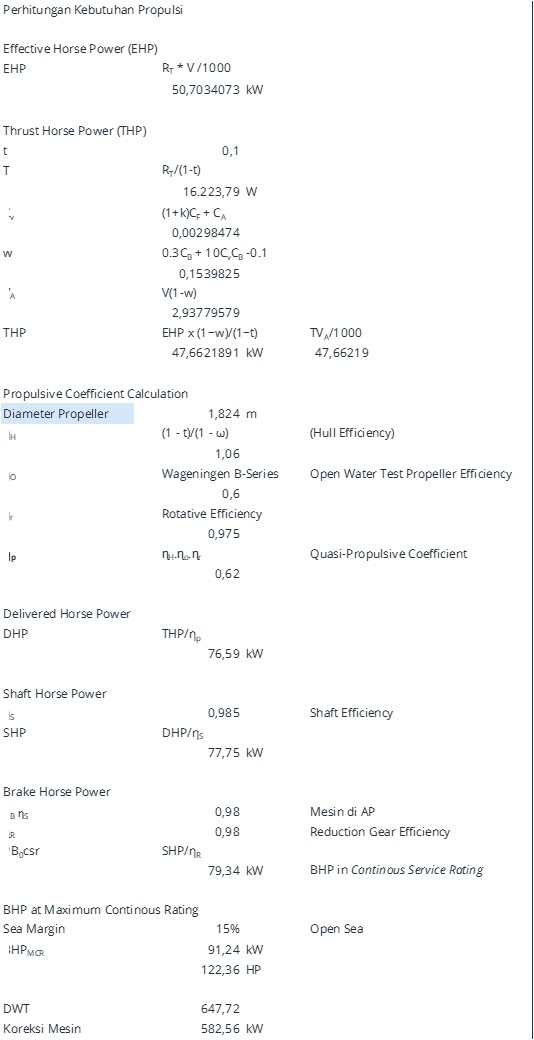
\includegraphics[width=\linewidth,height=\textheight,keepaspectratio]{lampiran/deskap-3.jpg}
    \caption*{Perhitungan Kebutuhan Propulsi}
\end{figure}

\begin{figure}[!ht]
    \centering
    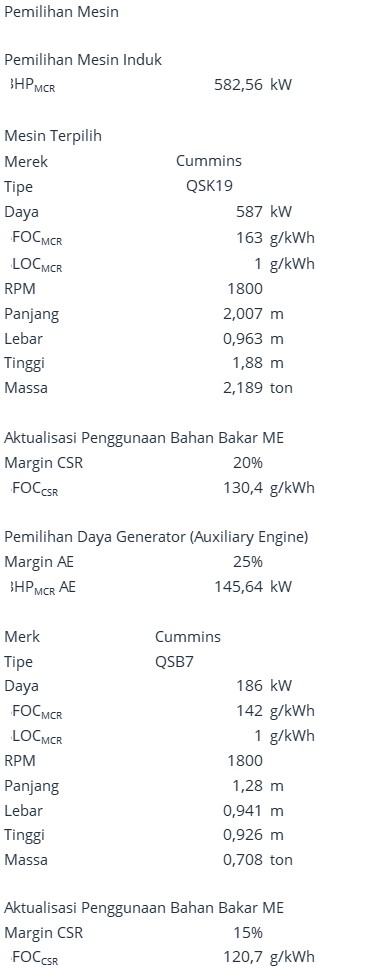
\includegraphics[width=\linewidth,height=\textheight,keepaspectratio]{lampiran/deskap-4.jpg}
    \caption*{Pemilihan Mesin}
\end{figure}

\begin{figure}[!ht]
    \centering
    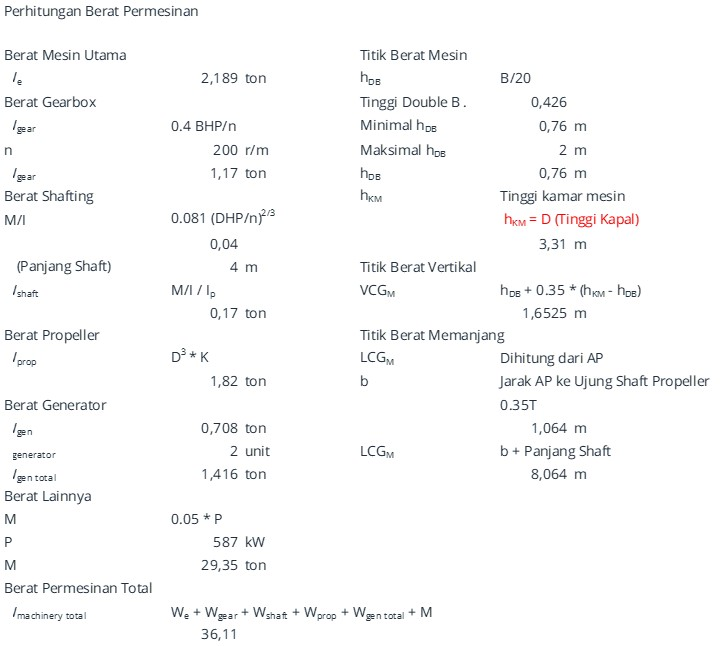
\includegraphics[width=\linewidth,keepaspectratio]{lampiran/deskap-5.jpg}
    \caption*{Perhitungan Berat Mesin}
\end{figure}

\begin{figure}[!ht]
    \centering
    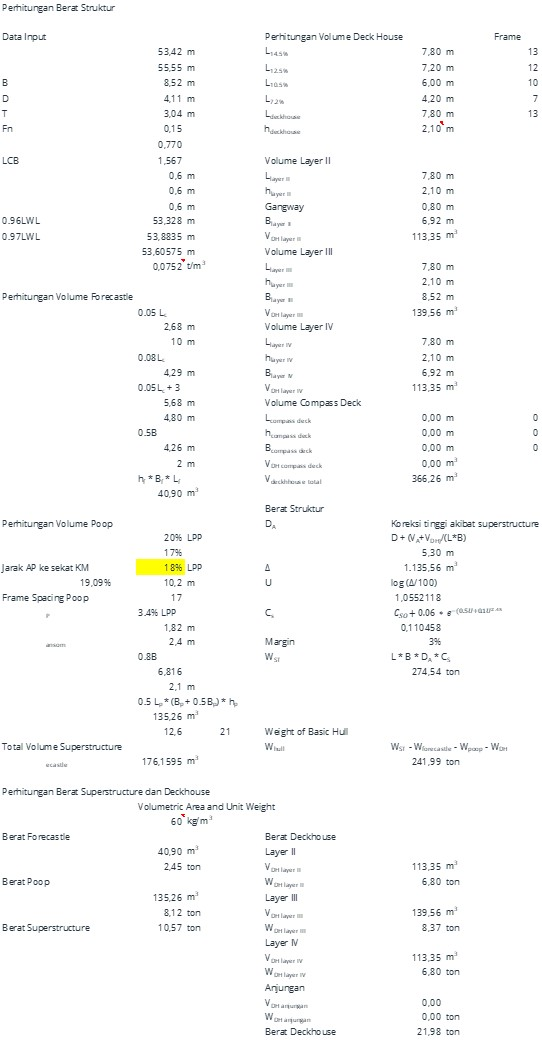
\includegraphics[width=\linewidth,height=\textheight,keepaspectratio]{lampiran/deskap-6.jpg}
    \caption*{Perhitungan Berat Struktur}
\end{figure}

\begin{figure}[!ht]
    \centering
    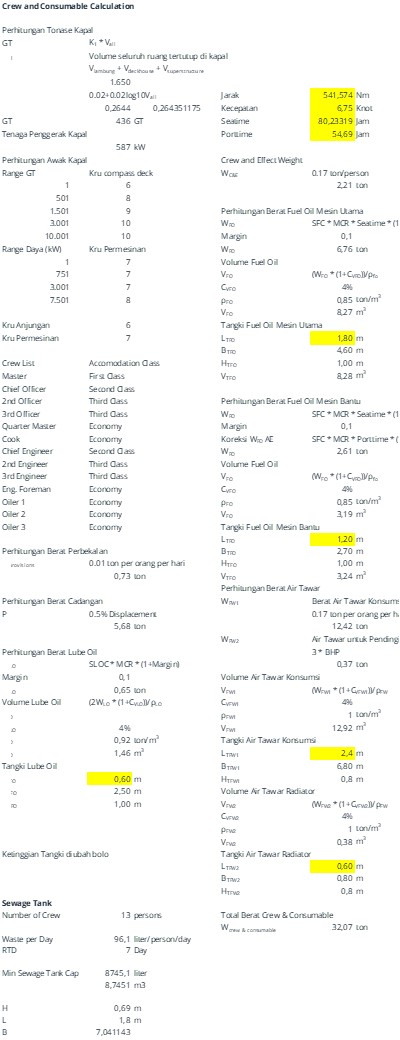
\includegraphics[width=\linewidth,height=\textheight,keepaspectratio]{lampiran/deskap-7.jpg}
    \caption*{Perhitungan \emph{Consumable} dan Crew}
\end{figure}

\begin{figure}[!ht]
    \centering
    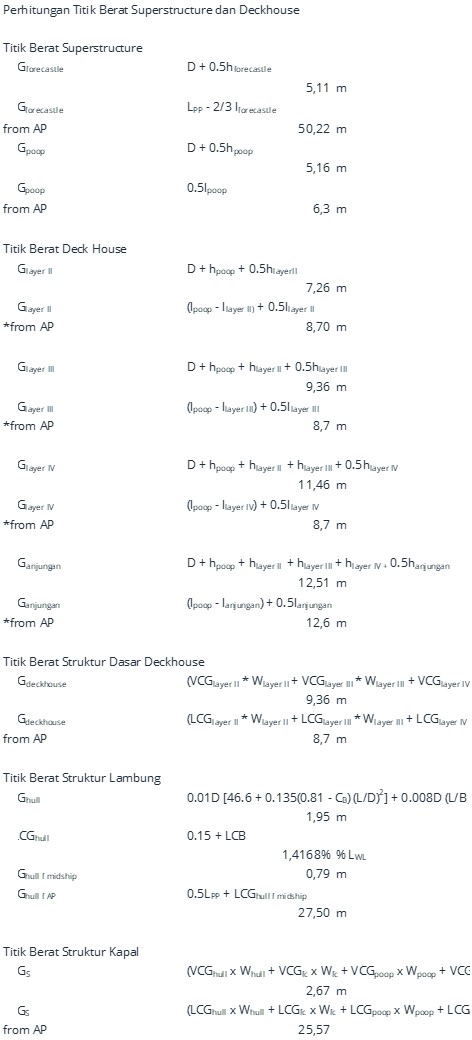
\includegraphics[width=\linewidth,height=\textheight,keepaspectratio]{lampiran/deskap-8.jpg}
    \caption*{Perhitungan Titik Berat \emph{Superstructure}}
\end{figure}

\begin{figure}[!ht]
    \centering
    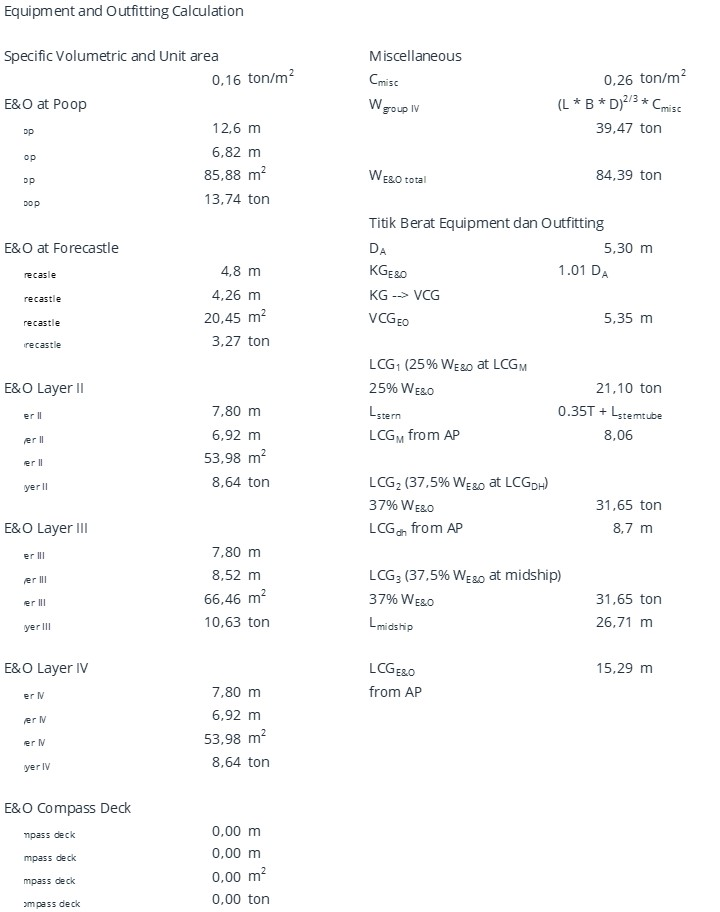
\includegraphics[width=\linewidth,keepaspectratio]{lampiran/deskap-9.jpg}
    \caption*{Perhitungan \emph{Equipment and Outfitting}}
\end{figure}

\begin{figure}[!ht]
    \centering
    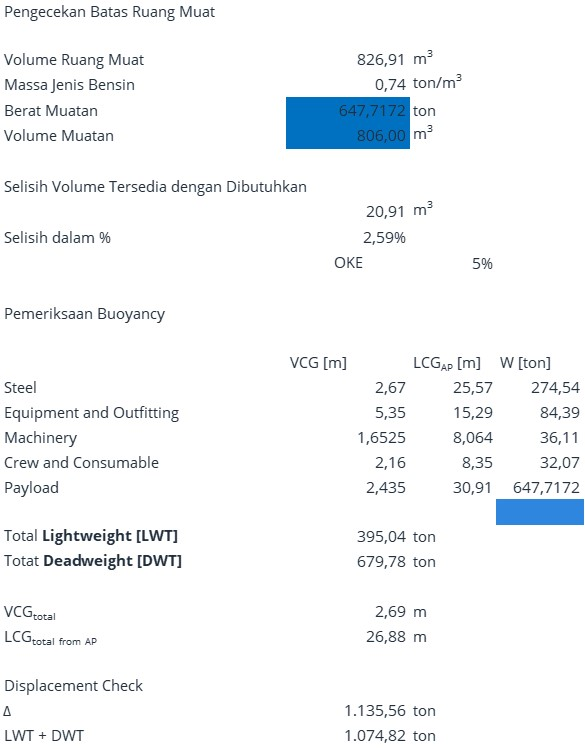
\includegraphics[width=\linewidth,keepaspectratio]{lampiran/deskap-10.jpg}
    \caption*{Pengecekan Batas Ruang Muat}
\end{figure}

\begin{figure}[!ht]
    \centering
    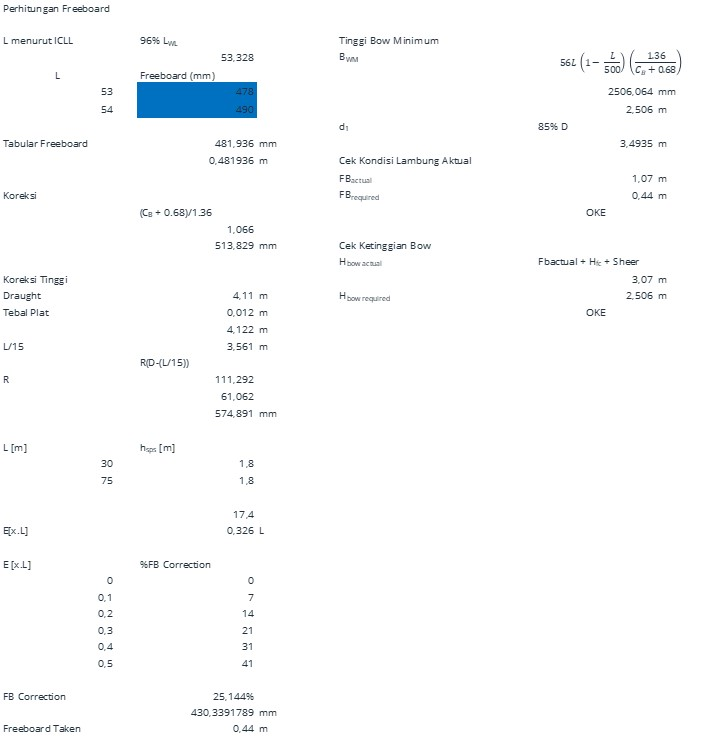
\includegraphics[width=\linewidth,keepaspectratio]{lampiran/deskap-11.jpg}
    \caption*{Perhitungan Lambung Timbul}
\end{figure}

\section*{Lampiran Tabel Simulasi}
\label{sec:lampiran-simulasi}

\begin{figure}[!ht]
    \centering
    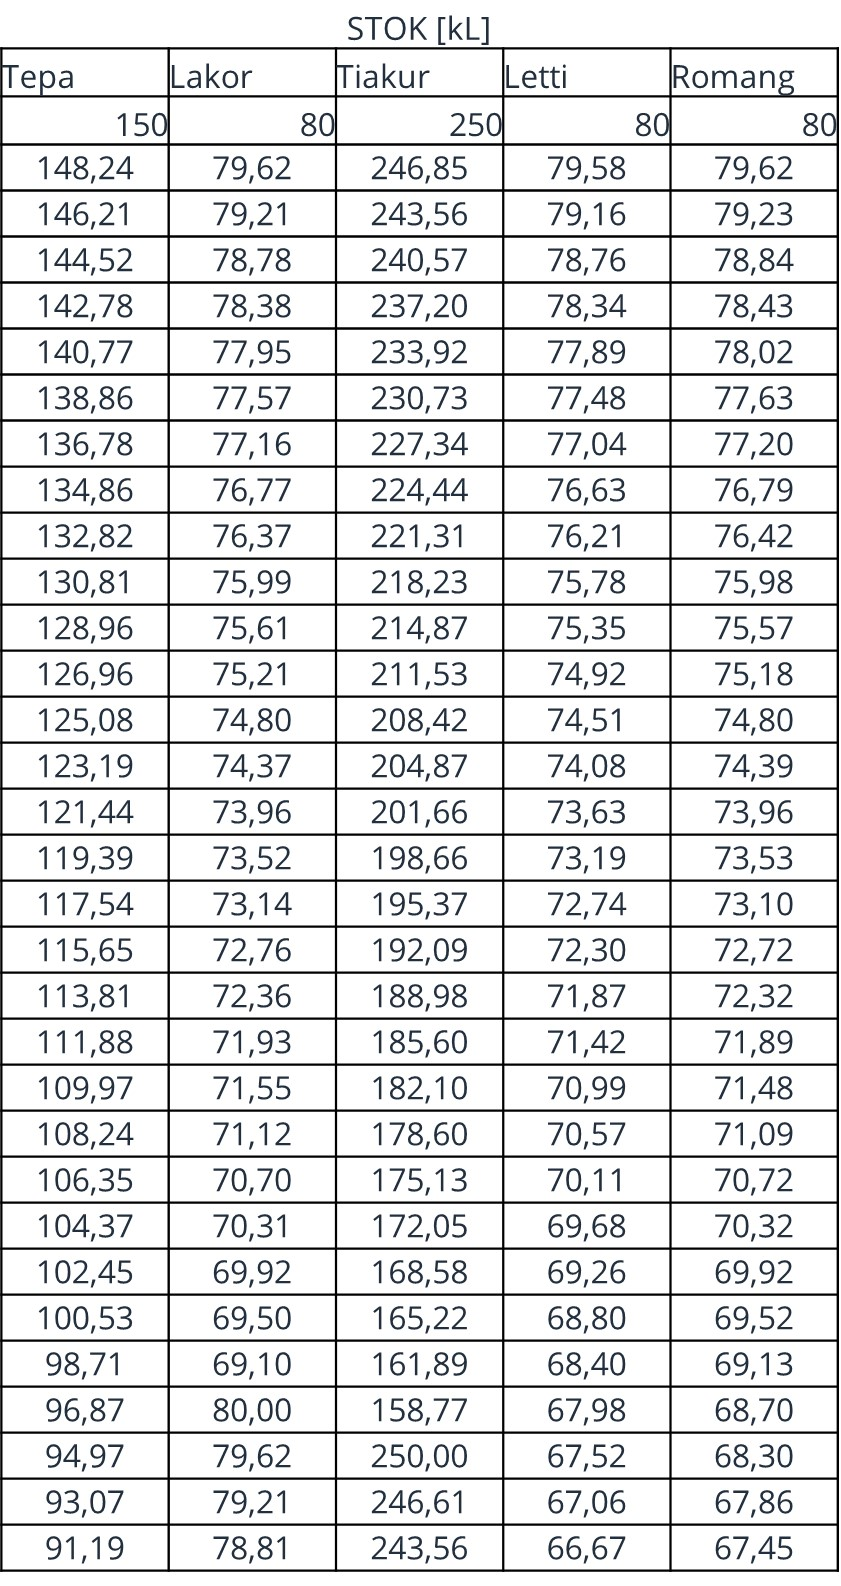
\includegraphics[width=\linewidth,height=\textheight,keepaspectratio]{lampiran/tabel-stok-simu.jpg}
    \caption*{Potongan Tabel Persediaan BBM}
\end{figure}

\begin{figure}[!ht]
    \centering
    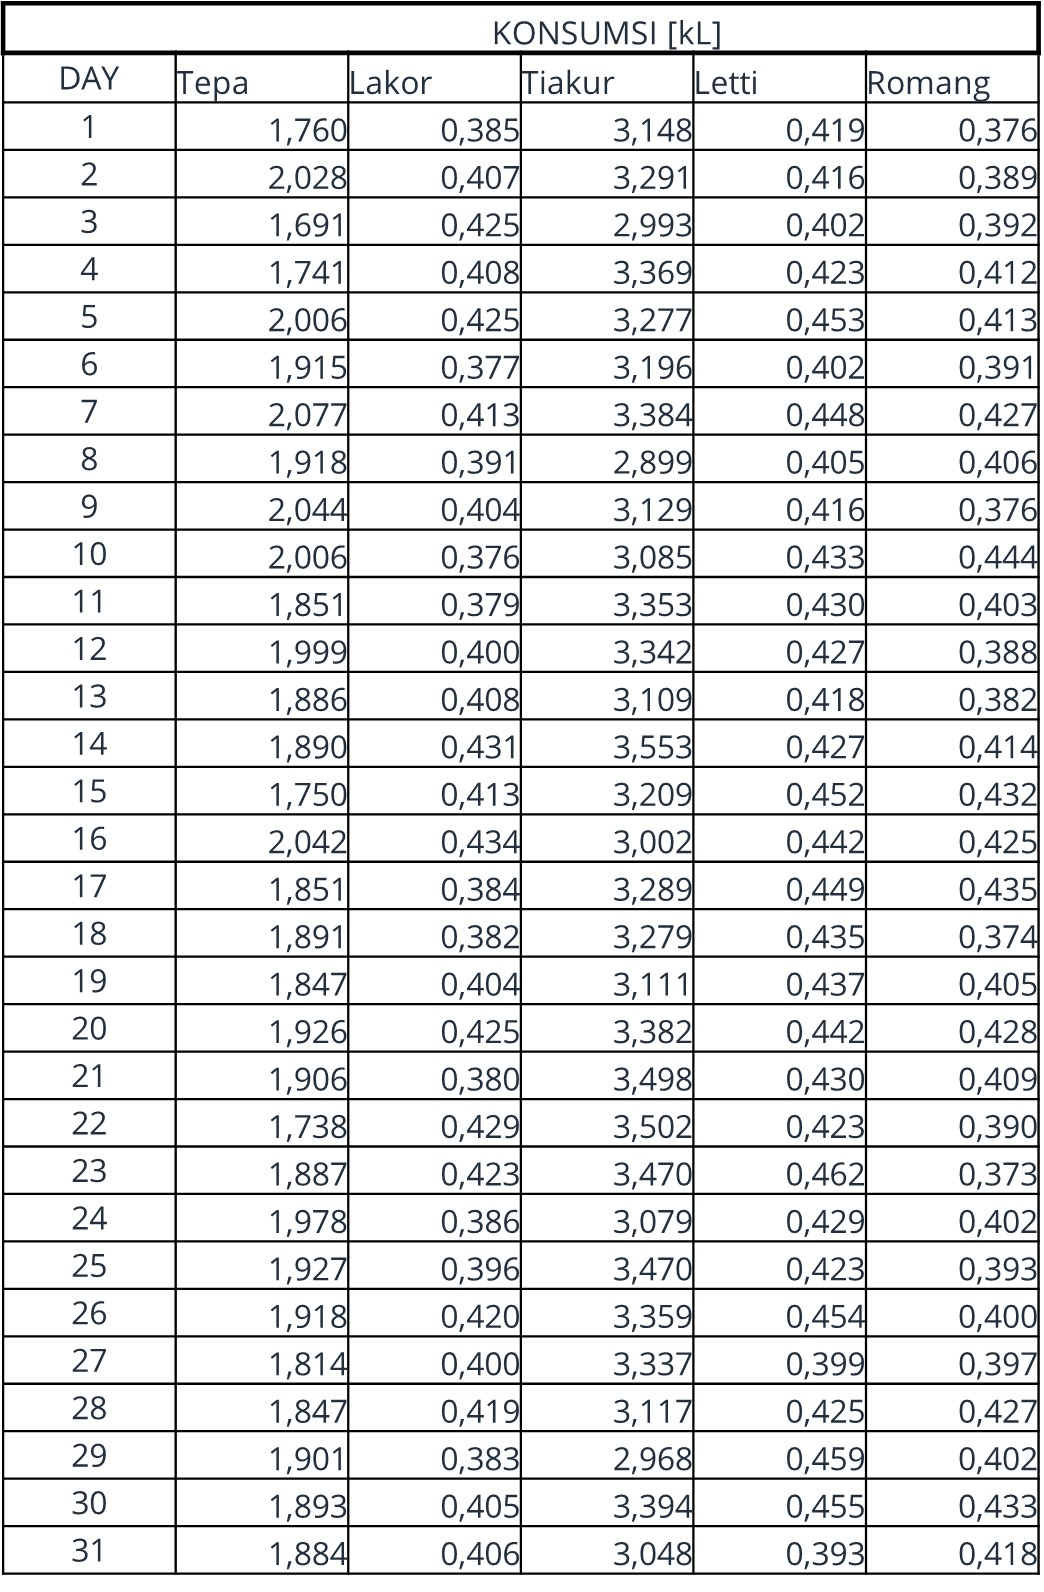
\includegraphics[width=\linewidth,height=\textheight,keepaspectratio]{lampiran/tabel-konsumsi-simu.jpg}
    \caption*{Potongan Tabel Variasi Konsumsi BBM Setiap Titik}
\end{figure}

\begin{figure}[!ht]
    \centering
    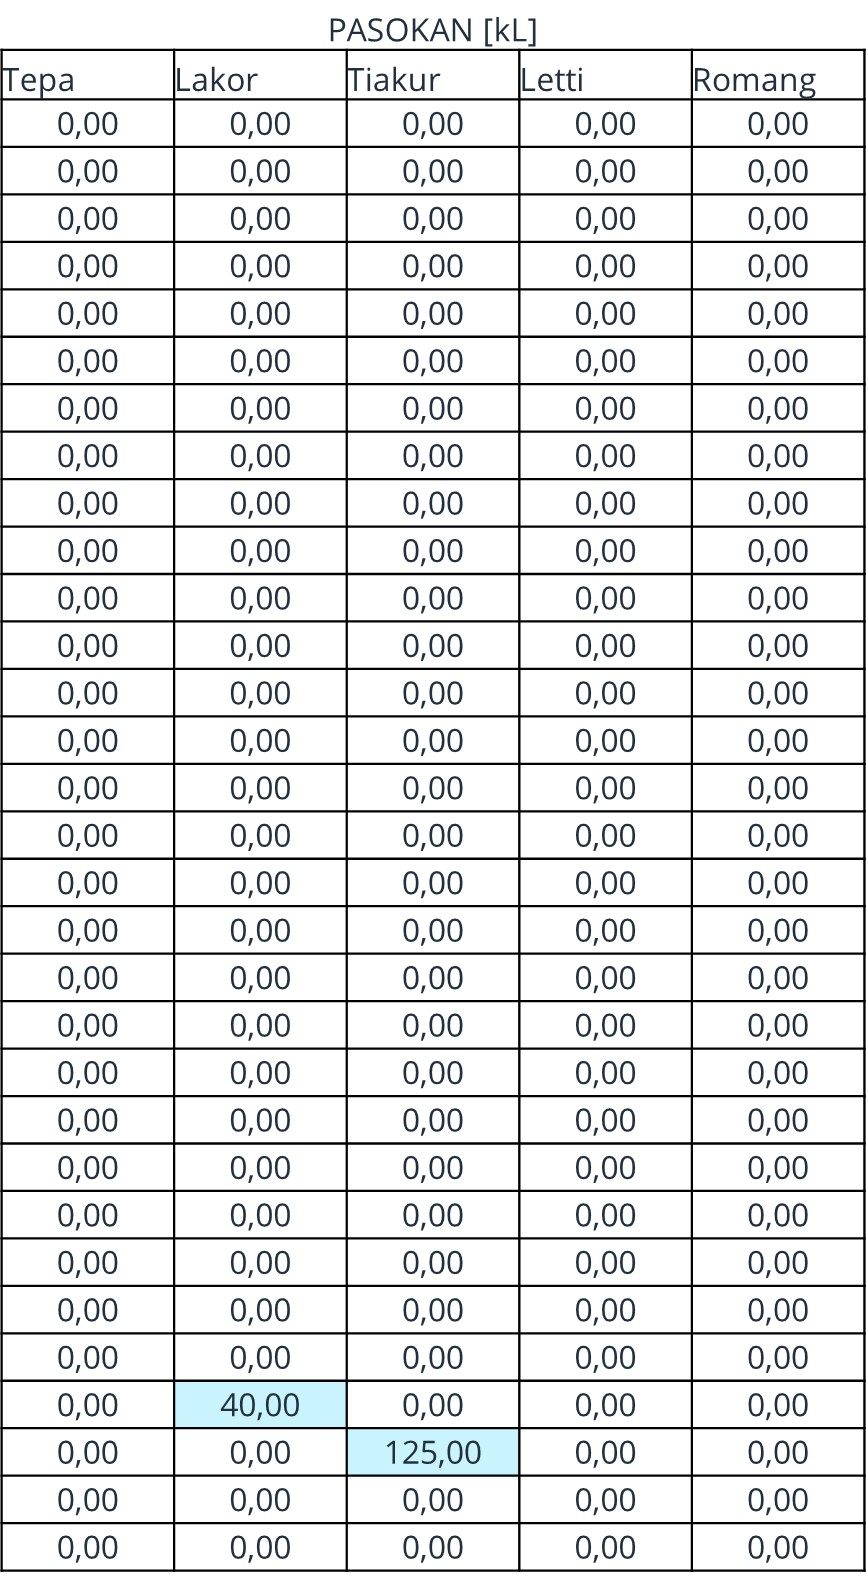
\includegraphics[width=\linewidth,height=\textheight,keepaspectratio]{lampiran/tabel-pasokan-simu.jpg}
    \caption*{Potongan Tabel Pemasokan BBM}
\end{figure}

\begin{sidewaysfigure}
    \centering
    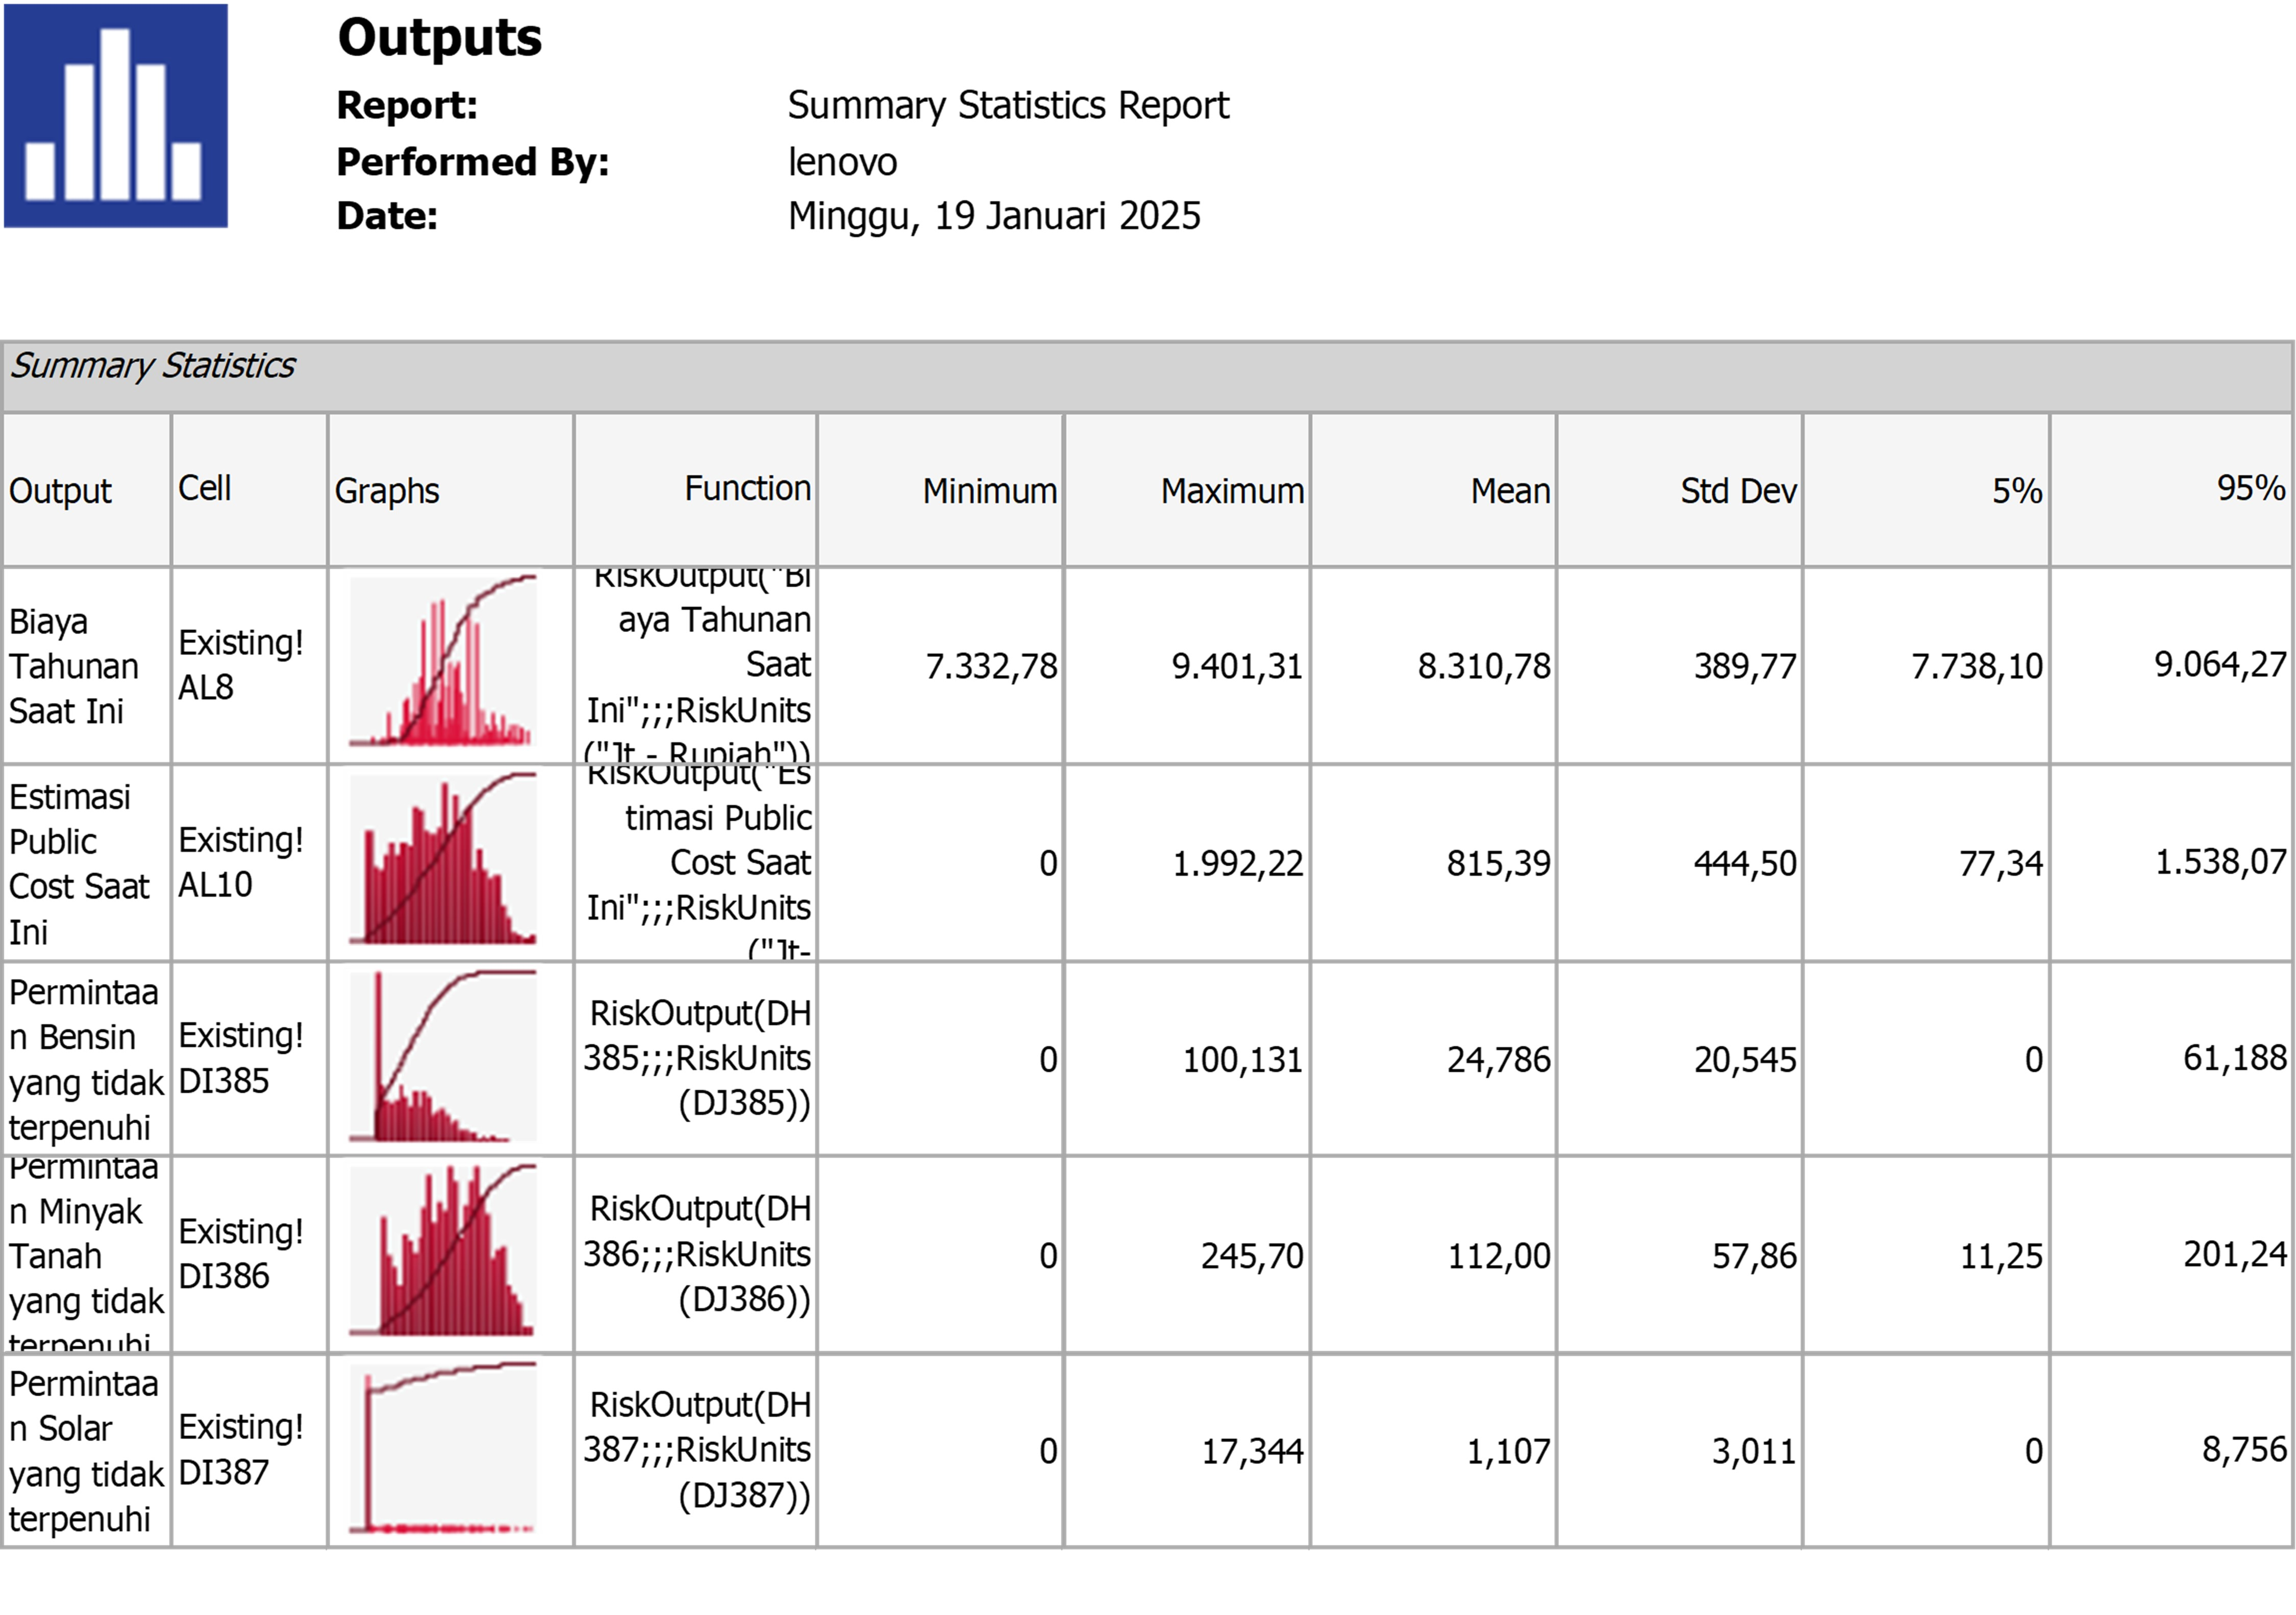
\includegraphics[width=\textwidth]{lampiran/summary-now.jpg}
    \caption*{\emph{Summary Statistics} Kondisi Saat Ini}
\end{sidewaysfigure}

\begin{figure}[!ht]
    \centering
    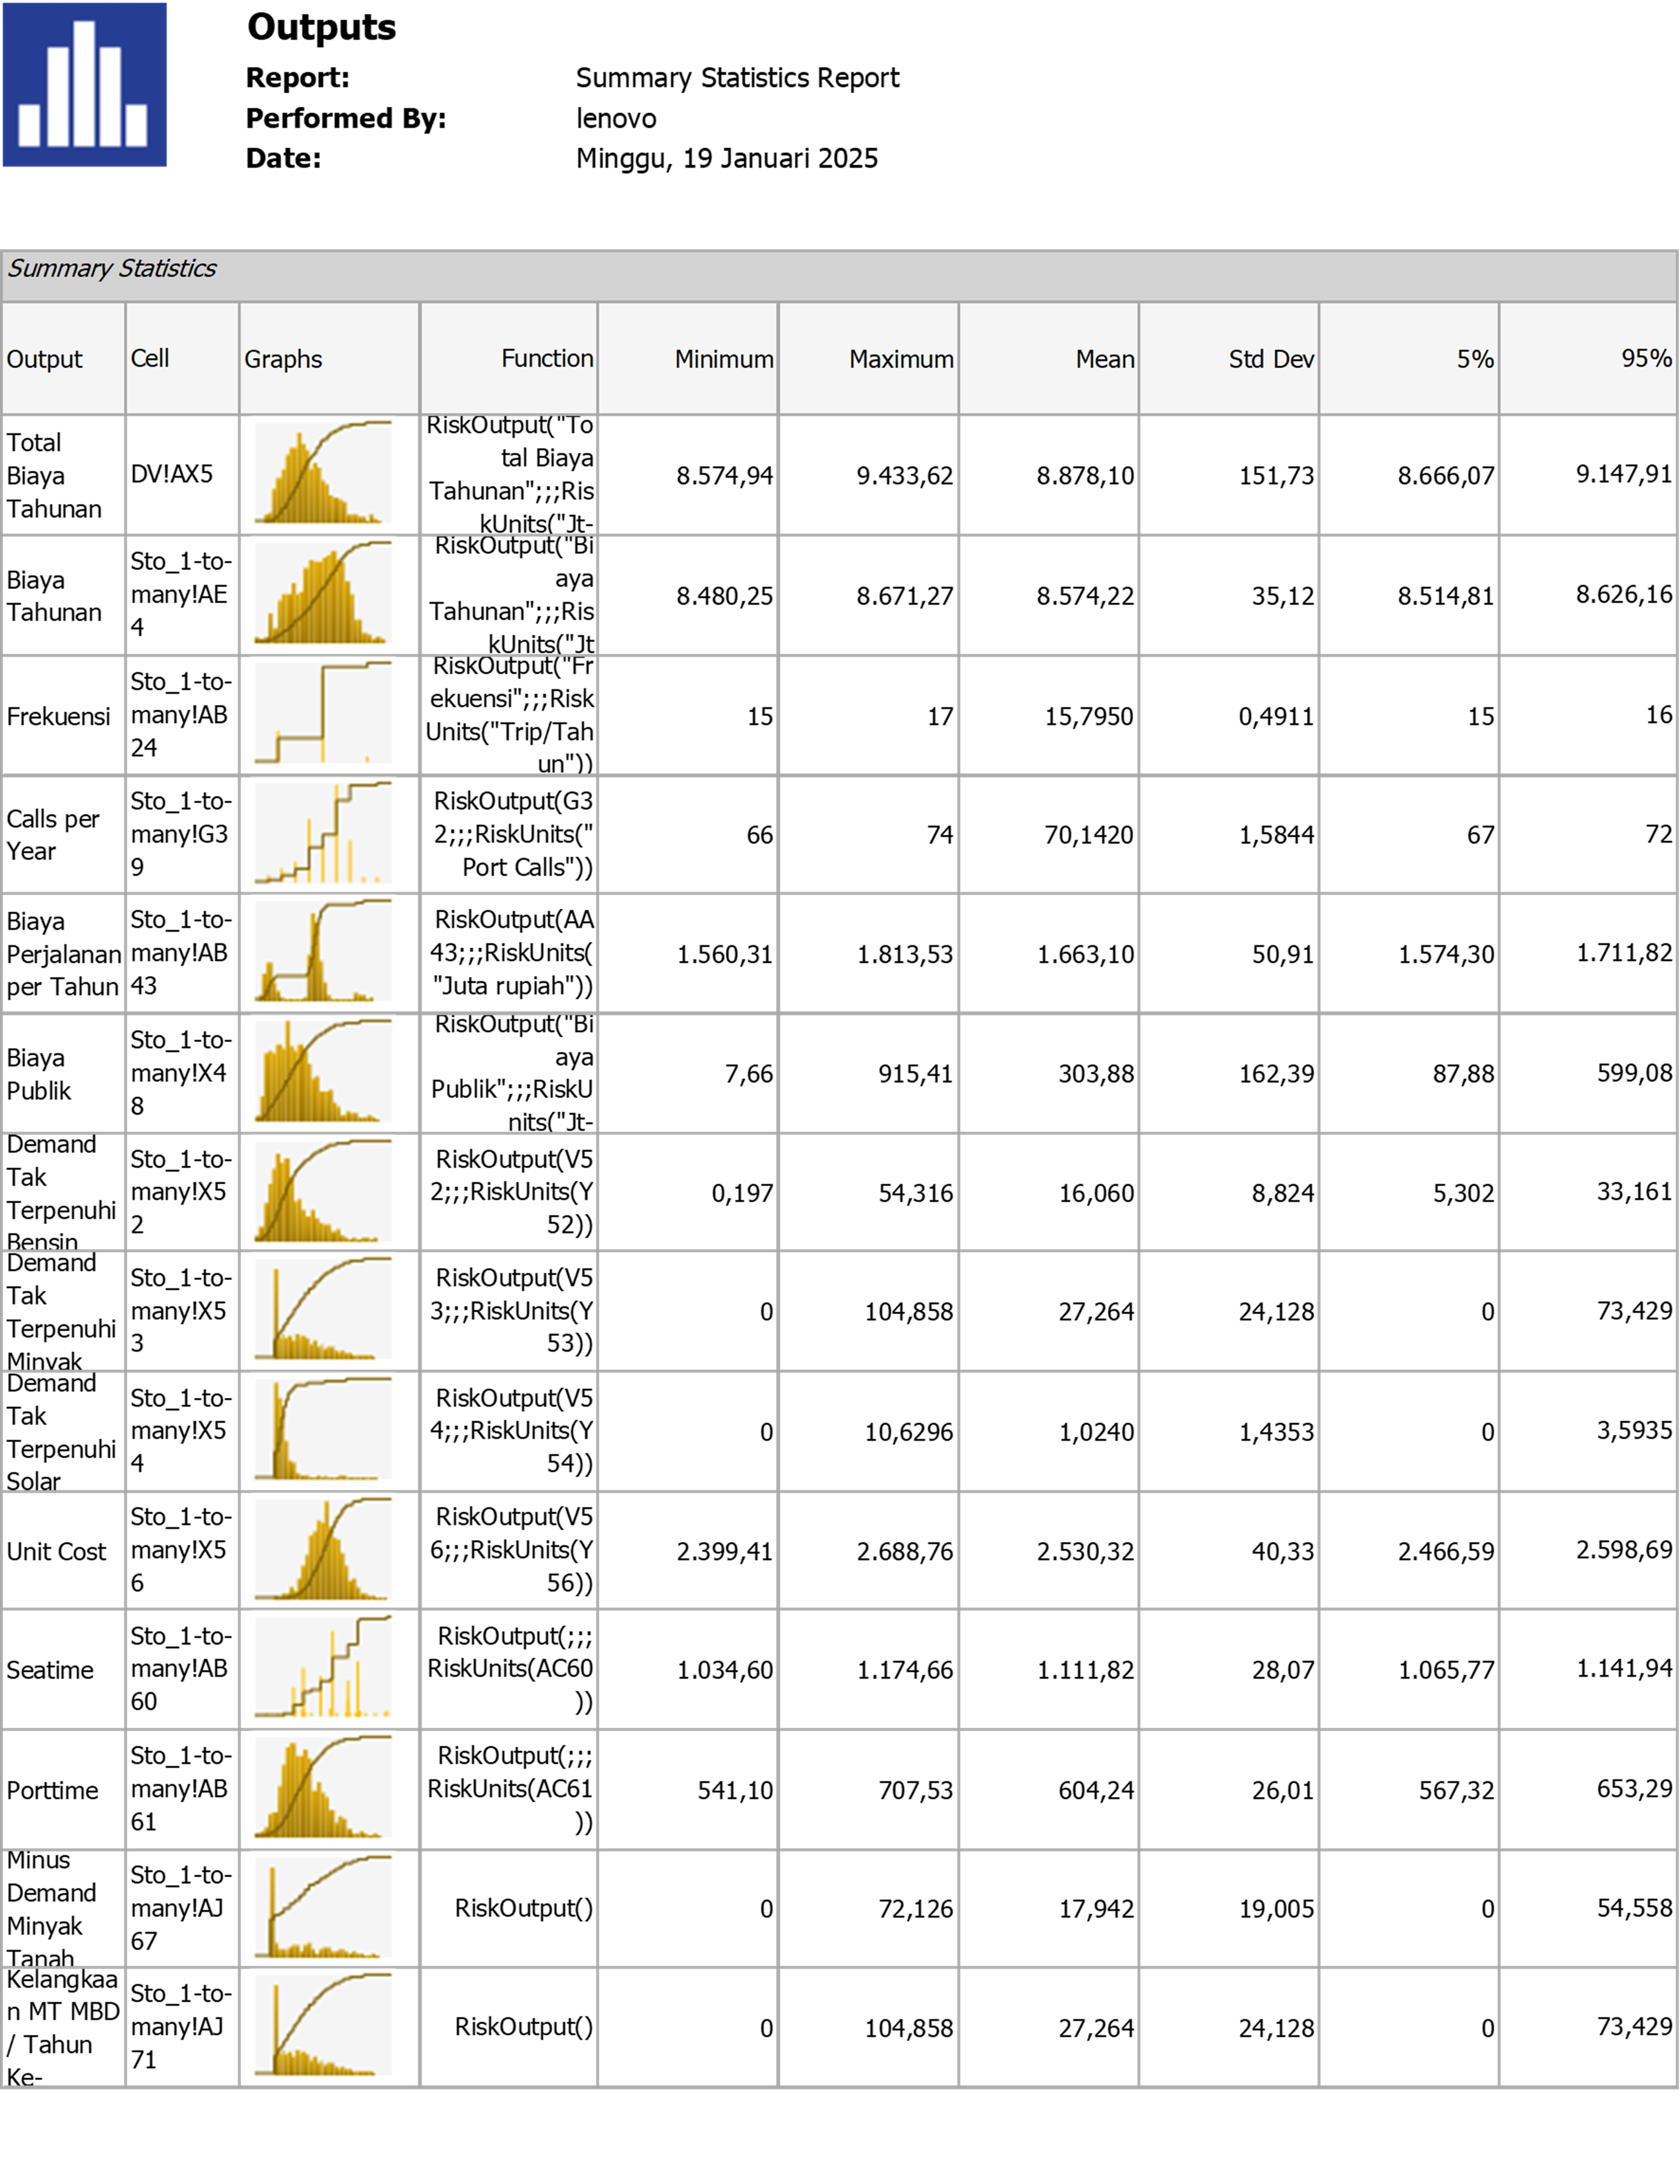
\includegraphics[width=\linewidth,height=\textheight,keepaspectratio]{lampiran/summary-no-tangki.jpg}
    \caption*{\emph{Summary Statistics} Sistem Baru Tanpa Tangki}
\end{figure}

\begin{figure}[!ht]
    \centering
    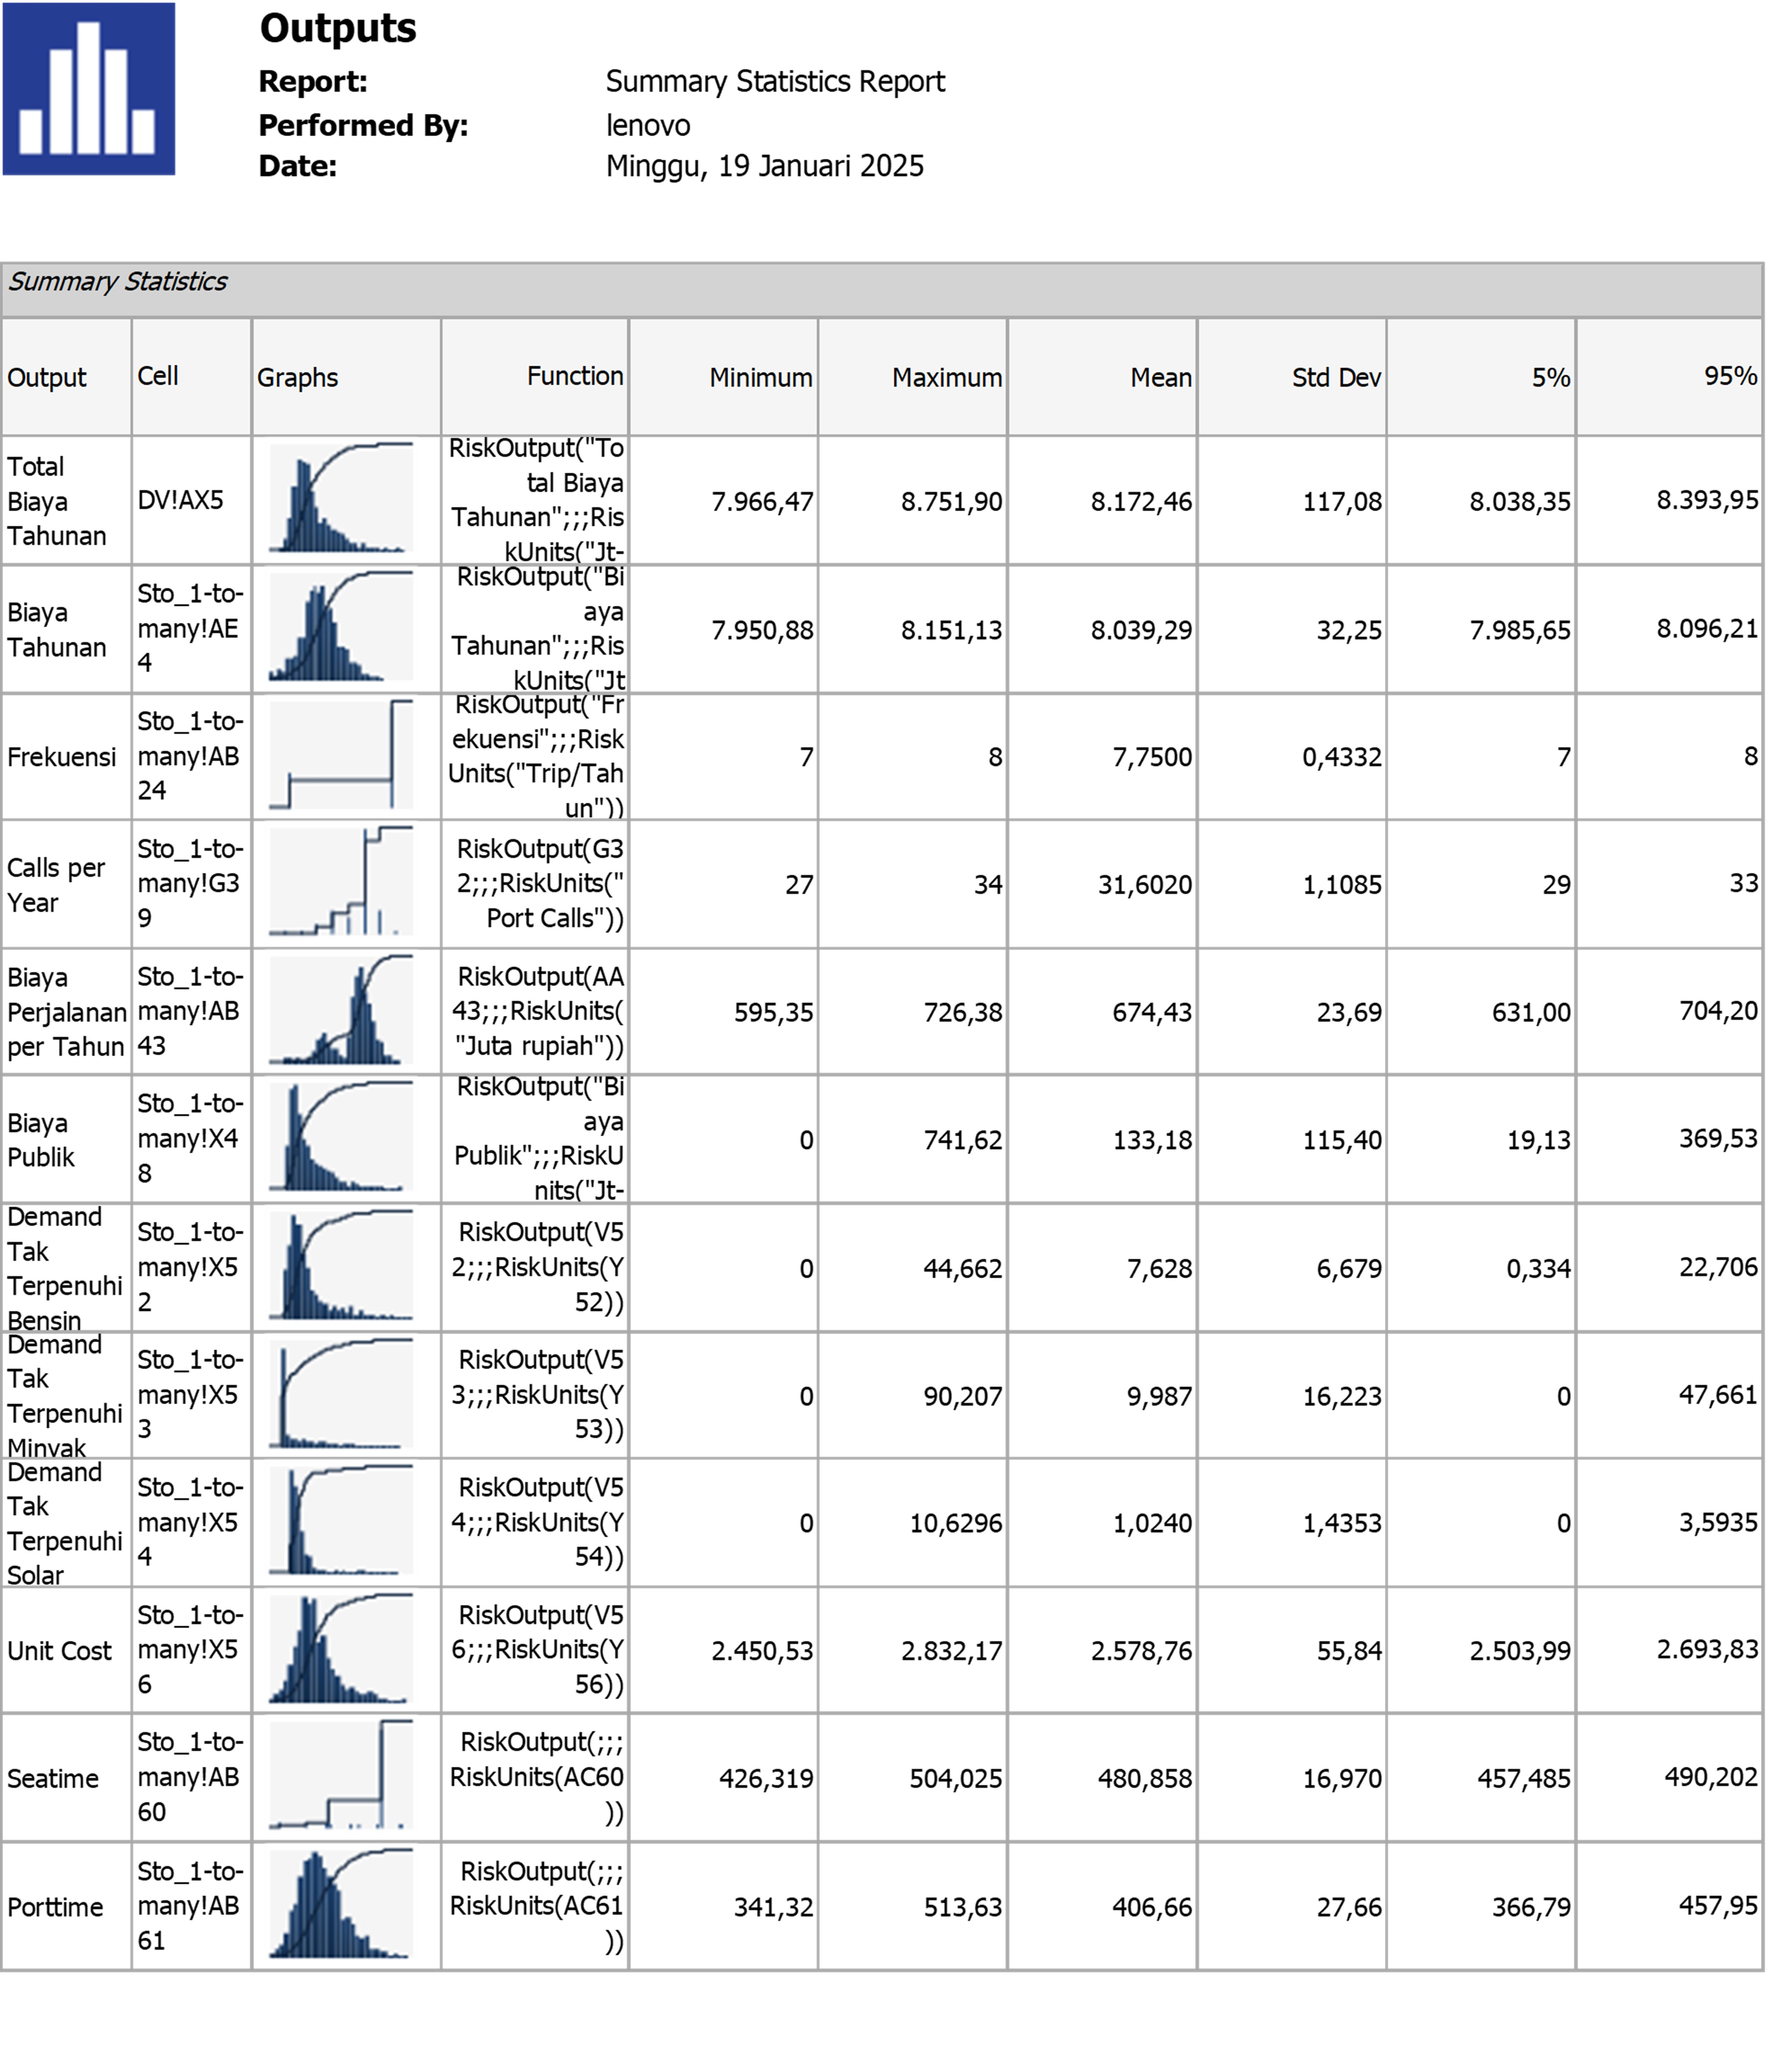
\includegraphics[width=\linewidth,height=\textheight,keepaspectratio]{lampiran/summary-tangki.jpg}
    \caption*{\emph{Summary Statistics} Sistem Baru Dengan Tangki}
\end{figure}